
\documentclass[a4paper,hidelinks,14pt]{extarticle}

%%% Поля и разметка страницы %%%
\usepackage{pdflscape}   % Для включения альбомных страниц
\usepackage{geometry} % Для последующего задания полей
\usepackage{setspace} % Для интерлиньяжа
\usepackage[14pt]{extsizes}
\usepackage{titlesec}
\usepackage{tocloft}
\usepackage{enumitem}
\usepackage{fancyhdr}
\usepackage{chngcntr} % Для нумерации параграфов
\usepackage{calc}     % Для расчета ширины элементов
\usepackage{url}      % Для настройки отображение ссылок
\usepackage{pdfpages} % Для встраивания PDF

%%% Кодировки и шрифты %%%
\usepackage{cmap}                    % Улучшенный поиск русских слов в полученном pdf-файле
\usepackage[T1,T2A]{fontenc}	     % Поддержка русских букв
\usepackage[utf8x]{inputenc}	     % Кодировка utf8
\usepackage[english, russian]{babel} % Языки: русский, английский

\usepackage{pscyr}						% Красивые русские шрифты

%%% Математические пакеты %%%
\usepackage{amsthm,amsfonts,amsmath,amssymb,amscd} % Математические дополнения от AMS

%%% Оформление абзацев %%%
\usepackage{indentfirst} % Красная строка

%%% Цвета %%%
\usepackage{color}

%%% Таблицы %%%
\usepackage{longtable}		     % Длинные таблицы
\usepackage{tabularx}
\usepackage{tabulary}
\usepackage{multirow,makecell,array} % Улучшенное форматирование таблиц

%%% Сноски %%%
\usepackage{tablefootnote} % Для сносок в таблицах
\usepackage{scrextend}

%%% Общее форматирование
\usepackage[tableposition=top]{caption}
\captionsetup[figure]{labelsep=space,justification=centering,singlelinecheck=false}
\captionsetup[lstlisting]{labelsep=space,justification=centering,singlelinecheck=false}

\usepackage{soul}                    % Поддержка переносоустойчивых подчёркиваний и зачёркиваний
\usepackage{multicol}

%%% Библиография %%%
\usepackage{cite} % Красивые ссылки на литературу

%%% Гиперссылки %%%
\usepackage[unicode,plainpages=false,pdfpagelabels=false]{hyperref}

%%% Изображения %%%
\usepackage{graphicx} % Подключаем пакет работы с графикой

%%% Листинги %%%
\usepackage{listings} %% собственно, это и есть пакет listings

%%% Рисунки TEX %%%
\usepackage{tikz}        % Подключаемые пакеты
%%% Язык текста %%%
\selectlanguage{russian}

%%% Кодировки и шрифты %%%
\renewcommand{\rmdefault}{ftm} % Включаем Times New Roman

%%% Макет страницы %%%
\geometry{a4paper,top=20mm,left=31mm,right=15mm,bottom=27mm}
\setstretch{1.05}

%%% Выравнивание и переносы %%%
\sloppy				% Избавляемся от переполнений
\clubpenalty=10000		% Запрещаем разрыв страницы после первой строки абзаца
\widowpenalty=10000		% Запрещаем разрыв страницы после последней строки абзаца
\interfootnotelinepenalty=10000 % Запрет разрывов сносок

%%% Настройки полей %%%

% Титульная страница
\fancypagestyle{empty}{%
\fancyhf{} % clear all header and footer fields
\renewcommand{\headrulewidth}{0pt}
\renewcommand{\footrulewidth}{0pt}
% \setlength{\footskip}{9mm}
\setlength{\headheight}{4mm}
}

% Основной текст
\fancypagestyle{plain}{%
\fancyhf{} % clear all header and footer fields
\fancyfoot[R]{\thepage}
\renewcommand{\headrulewidth}{0pt}
\renewcommand{\footrulewidth}{0pt}
\setlength{\footskip}{11mm}
\setlength{\headheight}{4mm}
}

\pagestyle{plain}

%%% Оформление текста

\setlength{\parskip}{0mm}
\setlength{\parindent}{1.25cm}
\raggedbottom{}

\renewcommand\floatpagefraction{.9}
\renewcommand\dblfloatpagefraction{.9} % for two column documents
\renewcommand\topfraction{.9}
\renewcommand\dbltopfraction{.9}       % for two column documents
\renewcommand\bottomfraction{.9}
\renewcommand\textfraction{.1}
\setcounter{totalnumber}{50}
\setcounter{topnumber}{50}
\setcounter{bottomnumber}{50}

%%% Оформление заголовков
\newcommand{\sectionbreak}{\clearpage}

\titleformat{\section}{\large\bfseries}{\thesection}{\wordsep}{}
\titlespacing*{\section}{\parindent}{\baselineskip}{\baselineskip}

\titleformat{name=\section,numberless}{\large\bfseries\filcenter}{}{0mm}{}
\titlespacing*{name=\section,numberless}{0mm}{\baselineskip}{\baselineskip}

\titleformat{name=\subsection}{\normalsize\bfseries}{\thesubsection}{\wordsep}{}
\titlespacing*{\subsection}{\parindent}{\baselineskip}{\baselineskip}

\titleformat{name=\subsection,numberless}{\normalsize\bfseries}{}{0mm}{}
\titlespacing*{name=\subsection,numberless}{0mm}{\baselineskip}{\baselineskip}

\titleformat{name=\subsubsection}{\normalsize\bfseries}{\thesubsubsection}{\wordsep}{}
\titlespacing*{\subsubsection}{\parindent}{\baselineskip}{\baselineskip}

\titleformat{name=\subsubsection,numberless}{\normalsize\bfseries}{}{0mm}{}
\titlespacing*{name=\subsubsection,numberless}{0mm}{\baselineskip}{\baselineskip}

\counterwithout{paragraph}{subsubsection}
\counterwithin{paragraph}{subsection}
\renewcommand{\theparagraph}{\thesubsection.\arabic{paragraph}}
\setcounter{secnumdepth}{4}

\titleformat{name=\paragraph}[runin]{\normalsize\bfseries}{\theparagraph}{\wordsep}{}
\titlespacing*{\paragraph}{\parindent}{\baselineskip}{\wordsep}

%%% Оформление списков
\setlist[1]{itemindent=1.85cm,leftmargin=0mm,itemsep=0mm,topsep=0mm,parsep=0mm}
\setlist[itemize,1]{label=---}
\setlist[enumerate,1]{label=\arabic*}

\setlist[2]{itemindent=3.1cm,leftmargin=0mm,itemsep=0mm,topsep=0mm,parsep=0mm}

% Cтиль для списков, на которые есть ссылки в тексте
\AddEnumerateCounter{\Asbuk}{\@asbuk}{\cyrm}
\newlist{reflist}{enumerate}{1}
\setlist*[reflist,1]{label=\asbuk*)}
\setlist*[reflist,2]{label=\asbuk*)}

%%% Оформление сносок

\deffootnote[1.65cm]{0mm}{1.25cm}{\textsuperscript{\thefootnotemark) }}
\renewcommand{\footnotesize}{\normalsize\selectfont}
\setlength{\footnotesep}{\parsep}

%%% Оформление ссылок
\urlstyle{same}

%%% Размеры текста формул %%%

\DeclareMathSizes{12}{12}{6}{4}

%%% Расстояние между формулами

\AtBeginDocument{%
  \setlength\abovedisplayskip{\baselineskip}%
  \setlength\belowdisplayskip{\baselineskip}%
  \setlength\abovedisplayshortskip{\baselineskip}%
  \setlength\belowdisplayshortskip{\baselineskip}%
}

%%% Расстояние между плавающими элементами

\setlength{\floatsep}{1.5\baselineskip plus 0mm minus 0mm}     % between top floats
\setlength{\textfloatsep}{1.5\baselineskip plus 0mm minus 0mm} % between top/bottom floats and text
\setlength{\intextsep}{1.5\baselineskip plus 0mm minus 0mm}    % between text and float
\setlength{\dbltextfloatsep}{1.5\baselineskip plus 0mm minus 0mm}
\setlength{\dblfloatsep}{1.5\baselineskip plus 0mm minus 0mm}

%% Нумерация плавающих элементов

\counterwithin{figure}{section}
\counterwithin{table}{section}
\counterwithin{equation}{section}

\makeatletter
\AtBeginDocument{%
\renewcommand{\thetable}{\thesection.\arabic{table}}
\renewcommand{\thelstlisting}{\thesection.\arabic{lstlisting}}
\renewcommand{\thefigure}{\thesection.\arabic{figure}}
\let\c@lstlisting\c@figure}
\makeatother

%% Подписи плавающих элементов

\fboxsep=4mm
\fboxrule=0.1mm

\captionsetup[figure]{
  labelsep=endash,
  justification=centering,
  singlelinecheck=false,
  position=bottom,
  parskip=\parskip,
  belowskip=-0.6\baselineskip,
  skip=1.4\baselineskip}

\captionsetup[table]{
  labelsep=endash,
  justification=raggedright,
  singlelinecheck=false,
  position=top,
  belowskip=-0.4\baselineskip,
  skip=0mm}

\captionsetup[longtable]{
  labelsep=endash,
  justification=raggedright,
  singlelinecheck=false,
  position=top,
  belowskip=0.4\baselineskip,
  skip=0mm}

\captionsetup[lstlisting]{
  labelsep=endash
}

\lstset{
basicstyle=\scriptsize\ttfamily,
numberstyle=\scriptsize\ttfamily,
keywordstyle=\bfseries,
commentstyle=\itshape,
numbers=left,
stepnumber=1,
frame=single,
resetmargins=true,
xleftmargin=7mm,
xrightmargin=2mm,
captionpos=b,
keepspaces=true,
breaklines=true,
aboveskip=1.6\baselineskip,
belowskip=1.4\baselineskip,
abovecaptionskip=1.2\baselineskip}

\renewcommand{\arraystretch}{1.5}

%%% Настройка размеров вертикальных отступов

\renewcommand{\smallskip}{\vspace{0.3\baselineskip}}
\renewcommand{\bigskip}{\vspace{0.8\baselineskip}}

%%% Содержание %%%
\renewcommand{\cfttoctitlefont}{\hfil \large\bfseries}

\setlength{\cftparskip}{0mm}
\setlength{\cftbeforesecskip}{0mm}
\setlength{\cftaftertoctitleskip}{\baselineskip}
\cftsetpnumwidth{4mm}

\renewcommand{\cftsecfont}{}
\renewcommand{\cftsecpagefont}{\normalsize}
\renewcommand{\cftsecleader}{\cftdotfill{\cftdotsep}}

\setlength{\cftsecindent}{0mm}
\setlength{\cftsecnumwidth}{4mm}

\setlength{\cftsubsecindent}{4mm}
\setlength{\cftsubsecnumwidth}{8mm}

\setlength{\cftsubsubsecindent}{12mm}
\setlength{\cftsubsubsecnumwidth}{12mm}

%%% Библиография %%%

\makeatletter
\bibliographystyle{sys/ugost2003} % Оформляем библиографию в соответствии с ГОСТ 7.1 2003

\let\oldthebibliography=\thebibliography
\let\endoldthebibliography=\endthebibliography
\renewenvironment{thebibliography}[1]{
  \begin{oldthebibliography}{#1}
    \setlength{\parskip}{0mm}
    \setlength{\itemsep}{0mm}
}
{
\end{oldthebibliography}
}
   % Пользовательские стили

\begin{document}

 %%% Переопределение именований %%%
\renewcommand{\abstractname}{Аннотация}
\renewcommand{\alsoname}{см. также}
\renewcommand{\appendixname}{Приложение}
\renewcommand{\bibname}{Литература}
\renewcommand{\ccname}{исх.}
\renewcommand{\chaptername}{Глава}
\renewcommand{\contentsname}{СОДЕРЖАНИЕ}
\renewcommand{\enclname}{вкл.}
\renewcommand{\figurename}{Рисунок}
\renewcommand{\lstlistingname}{Рисунок}
\renewcommand{\headtoname}{вх.}
\renewcommand{\indexname}{Предметный указатель}
\renewcommand{\listfigurename}{Список рисунков}
\renewcommand{\listtablename}{Список таблиц}
\renewcommand{\pagename}{Стр.}
\renewcommand{\partname}{Часть}
\renewcommand{\seename}{см.}
\renewcommand{\tablename}{Таблица}
\renewcommand{\refname}{СПИСОК ИСПОЛЬЗОВАННЫХ ИСТОЧНИКОВ}
	 % Переопределение именований
\begin{titlepage}
\thispagestyle{empty}
\setlength{\parindent}{0ex} % set paragraph indenting to zero

\begin{center}
    Министерство образования Республики Беларусь \\
    \vspace{0.5ex}
    Учреждение образования \\
    БЕЛОРУССКИЙ ГОСУДАРСТВЕННЫЙ УНИВЕРСИТЕТ \\
    ИНФОРМАТИКИ И РАДИОЭЛЕКТРОНИКИ \\
    \vspace{0.5ex}
    Факультет Информационных Технологий и Управления \\
    \vspace{0.5ex}
    Кафедра ИТАС
\end{center}

\vspace{50mm}

\begin{center}
    Отчет по лабораторной работе №2 \\
    «МНОГОМЕРНЫЕ РАСПРЕДЕЛЕНИЯ ТЕОРИИ ВЕРОЯТНОСТЕЙ И МАТЕМАТИЧЕСКОЙ СТАТИСТИКИ»
\end{center}

\vspace{50mm}

\begin{minipage}{.4\linewidth}
    Выполнили \\
    студенты группы 820601

    \smallskip

    Проверил
\end{minipage}
\hfill
\begin{minipage}{.4\linewidth}
    \begin{flushright}
        Пальчик А. В.\\
        Шведов А. Р.

        \smallskip

        Ярмолик В. И.
    \end{flushright}
\end{minipage}

\vfill
\begin{center}
  Минск \the\year{}
\end{center}

\setlength{\parindent}{1.25cm} % reset paragraph indenting
\end{titlepage}
	 % Титульный лист
\setcounter{page}{2} % title and task pages

\tableofcontents

     % Содержание


% Введение
\section*{ВВЕДЕНИЕ}
\addcontentsline{toc}{section}{Введение}


Сайт, или веб-сайт (читается [вэбсайт], от англ. \textit{website: web} — «паутина, сеть» и \textit{site} — «место», буквально «место, сегмент, часть в сети»), — совокупность логически связанных между собой веб-страниц; также место расположения контента сервера. Обычно сайт в Интернете представляет собой массив связанных данных, имеющий уникальный адрес и воспринимаемый пользователем как единое целое. Веб-сайты называются так, потому что доступ к ним происходит по протоколу \textit{HTTP}.

Данная лабораторная работа рассматривает процесс разработки простейших сайтов на \textit{HTML}.



 % Цели работы
\section[Постановка задачи]{ПОСТАНОВКА ЗАДАЧИ}
Данная лабораторная работа ставит своей целью дать понимание принципов создания сайтов с помощью языка разметки \textit{HTML} и каскадных стилей \textit{CSS}. Конечной целью является создание сайта, содержащего \textit{8} страниц на языке \textit{HTML} согласно теме  «Погода на планете».


%\section{ТЕОРЕТИЧЕСКИЕ СВЕДЕНИЯ}

Тоже опциональный раздел, в нем излагаются, опять-таки, копипасты из методы либо
дополнительной литературы.
Может содержать картинки, формулы, таблицы\dots, всё это надо оформлять
в соответствии со стандартом.

В СТП есть указание на допустимые размеры рисуков (92 x 150 мм либо 150 x 240 мм),
кроме этого, рисунки должны быть отделены от прочих элементов страницы пробельной строкой:

  \begin{figure}[htbp]
    \centering
    
\includegraphics[width=150mm,height=92mm]{fig/scheme_p}
    \caption{Картинка для контроля отступов}
  \end{figure}

Допускается использовать сквозную нумерацию формул, рисунков, таблиц, листингов (как в этом макета),
можно также нумеровать плавающие элементы страницы в рамках раздела, к которому они принадлежат.
      % Теоретические сведения
\section[Теоретические сведения]{ТЕОРЕТИЧЕСКИЕ СВЕДЕНИЯ}

\subsection{Язык разметки HTML}
\textit{HTML} (\textit{HyperText Markup Language} — «язык гипертекстовой разметки») — стандартизированный язык разметки документов во Всемирной паутине. Большинство веб-страниц содержат описание разметки на языке \textit{HTML} (или \textit{XHTML}). Язык \textit{HTML} интерпретируется браузерами; полученный в результате интерпретации форматированный текст отображается на экране монитора компьютера или мобильного устройства.

\subsubsection{HTML-теги для работы со ссылками}
Следует знать о том, что все-таки главное предназначение языка \textit{HTML} –  создание гиперссылок. Гиперссылки создаются с помощью тэга \textit{<a>} и \textit{</a>} (от англ. \textit{anchor} – якорь). Сослаться  (перейти) к другому файлу (другой странице)  можно с помощью тэга <\textit{a href}=”ссылка на \textit{URL}”> элемент привязки </\textit{a}>.

Другая навигация по сайту:
\begin{itemize}
    \item <\textit{base}> Инструктирует браузер относительно полного базового адреса текущего документа.
    \item <\textit{nav}> Группирует ссылки навигации по сайту.
    \item <\textit{noindex}> Запрещает поисковой системе Яндекс индексировать текст и другие элементы внутри <\textit{noindex}>.
\end{itemize}


\subsubsection{HTML-теги для работы с изображениями}

Что понимается под словом «изображение»?  Изображение – это прежде всего файл, в котором хранится информация в графическом виде определенного формата. Обычно для веб-документов используются растровые (векторные форматы изображений мы рассмотрим позже в разделе, посвященном графике) графические форматы: \textit{GIF}, \textit{JPEG}, \textit{PNG}, \textit{BMP}.

В \textit{HTML} за работу с изображениями отвечают следующие тэги:
\begin{itemize}
    \item <\textit{img}> Отображает на веб-странице изображение.
    \item <\textit{map}> Служит контейнером для элементов <\textit{area}>, которые определяют активные области для карт-изображений.
    \item <\textit{picture}> Представляет собой контейнер для хранения нескольких элементов <\textit{source}>, которые поддерживают элемент <\textit{img}>. Это позволяет указывать разные изображения с учётом размера экрана, плотности пикселей, формата изображения и других параметров.

\end{itemize}




\subsection{Каскадные таблицы стилей CSS}
\textit{CSS} (\textit{Cascading Style Sheets }— каскадные таблицы стилей) — формальный язык описания внешнего вида документа, написанного с использованием языка разметки. Это язык иерархических правил, используемый для представления внешнего вида документа, написанного на \textit{HTML} или \textit{XML} (включая различные языки \textit{XML}, такие как \textit{SVG} и \textit{XHTML}). \textit{CSS} описывает каким образом элемент должен отображаться на экране, на бумаге, голосом или с использованием других медиа средств.

Преимущественно используется как средство описания, оформления внешнего вида веб-страниц, написанных с помощью языков разметки \textit{HTML} и \textit{XHTML}, но может также применяться к любым \textit{XML}-документам, например, к \textit{SVG} или \textit{XUL}.


\subsection{Предлагаемая реализация}
Реализуем страницу \textit{index.html} согласно Варианту -- «Погода на планете». Так же добавим дополнительно \textit{7} страниц, согласно заданию:
\begin{enumerate}
	\item Cтраница – «\textit{World}». Погода в мире;
   	\item Cтраница – «\textit{US}»;
    \item Cтраница – «\textit{Asia}»;
    \item Cтраница – «\textit{Africa}»;

    \item Cтраница – «\textit{Weather history}»;
    \item Cтраница – «\textit{Climate change}»;
    \item Форма обратной связи.
\end{enumerate}


Это реализовано в виде  верхней панели навигации, так же реализованы ссылки на метеорологические условия списка стран.


%\section{ХОД РАБОТЫ}

Это самый важный и объёмный раздел работы. Уважающие себя студенты пишут его самостоятельно.
Хорошо написан ход работы --- считай, лаба наполовину сдана!

\subsection{Примеры оформления формул}

В соответствии со стандартом \textbf{требуется нумеровать все 
формулы}, которые расположены на отдельных строках; в крайнем случае допускается нумеровать
группы однотипных формул, при этом про необходимость ссылок на эти формулы в тексте ничего не сказано.

Еще одна тонкость: \textbf{ссылки на формулы должны быть заключены в скобки}, вот так: смотри выражение ~\eqref{eq:observational_error}.
\begin{equation}
  \label{eq:observational_error}
  \gamma_{i} = \dfrac{\Delta_{i}}{X_{N}}*100\;\%,
\end{equation}

\noindent где\hspace{1em}$ X_{N} $ --- нормируемое значение, которое согласно ГОСТ 8.401-80
следует выбирать равным пределу измерения;

$ Q $ --- действительное значение величины;

$ X_{i} $ --- показание прибора.
\begin{equation}
  \label{eq:BaseOpt}
  \begin{aligned}
    E &= 8(20x_{11} + 25x_{12}) + 7(28x_{21} + 18x_{22}) \rightarrow \max = \\
    &= 160x_{11} + 200x_{12} + 196x_{21} + 126x_{22} \rightarrow \max.
  \end{aligned}
\end{equation}
\begin{equation}
  \label{eq:BaseNSM}
    \begin{aligned}
      E = 160x_{11} + 200x_{12} &+ 196x_{21} + 126x_{22} \rightarrow \max, \\
      20x_{11} &+ 25x_{12} \ge 20, \\
      28x_{21} &+ 18x_{22} \ge 6, \\
      x_{11} &+ x_{21} \le 0{,}8, \\
      x_{12} &+ x_{22} \le 0{,}6, \\
      x_{ij} & \ge 0, i, j = 1, 2.
    \end{aligned}
\end{equation}
Дальше идет какой-то текст\dots

\newpage

\subsection{Пример оформления листинга}

По сути, листинг рассматривается в тексте документа как нечто среднее между рисунком и таблицей. Поправьте меня, если что не так: 
\begin{lstlisting}[language=c,caption=Исходный код какой-то программы на C]
#include <stdio.h>

int main() /* prints "Hello world!" */
{ 
  printf("Hello world!"); 
  return 0;
}
\end{lstlisting}
Так как листинг формально является рисунком, важно, чтобы расстояние
между этим <<рисунком>> и текстом составляло ровно одну пробельную строку.
     % Ход работы
\section[Ход работы]{ХОД РАБОТЫ}

\subsection{Структура проекта}
В директории проекта были создан файл\textit{ index.html }который будет являться домашней страницей сайта, файлы остальных страниц находятся в той же директории.


\subsection{Каскадные стили}

Для создания стиля сайта был использован \textit{CSS}. Для этого в директории был создан файл .\textit{style.css}, который содержит в себе задание кастомных цветов и шрифтов для блоков и элементов, используемых в \textit{HTML}-коде страниц.

Так например был задан шрифт \textit{Helvetica} для любого блока .\textit{content}: рисунок~\ref{fig:fig2}.

\begin{figure}[htbp]
    \centering
    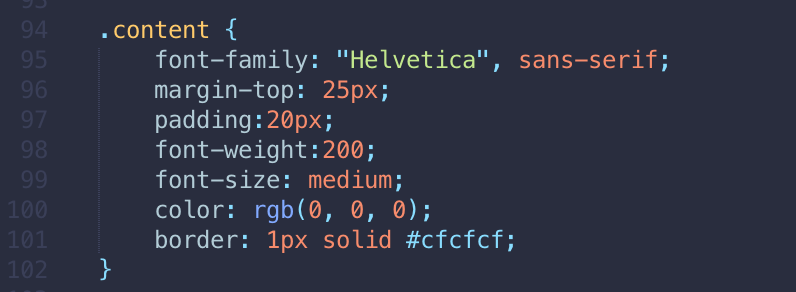
\includegraphics{fig/css.png}
    \caption{Использование каскадных стилей}
    \label{fig:fig2}
\end{figure}
\subsection{Панель навигации}
Для создания панели навигации воспользуемся элементом \textit{header} языка разметки \textit{HTML}, в него поместим ссылки на нужные страницы. Данная панель вставляется в каждую страницу. Програмная реализация предоставлена на рисунке~\ref{fig:fig1}.

\begin{figure}[htbp]
    \centering
    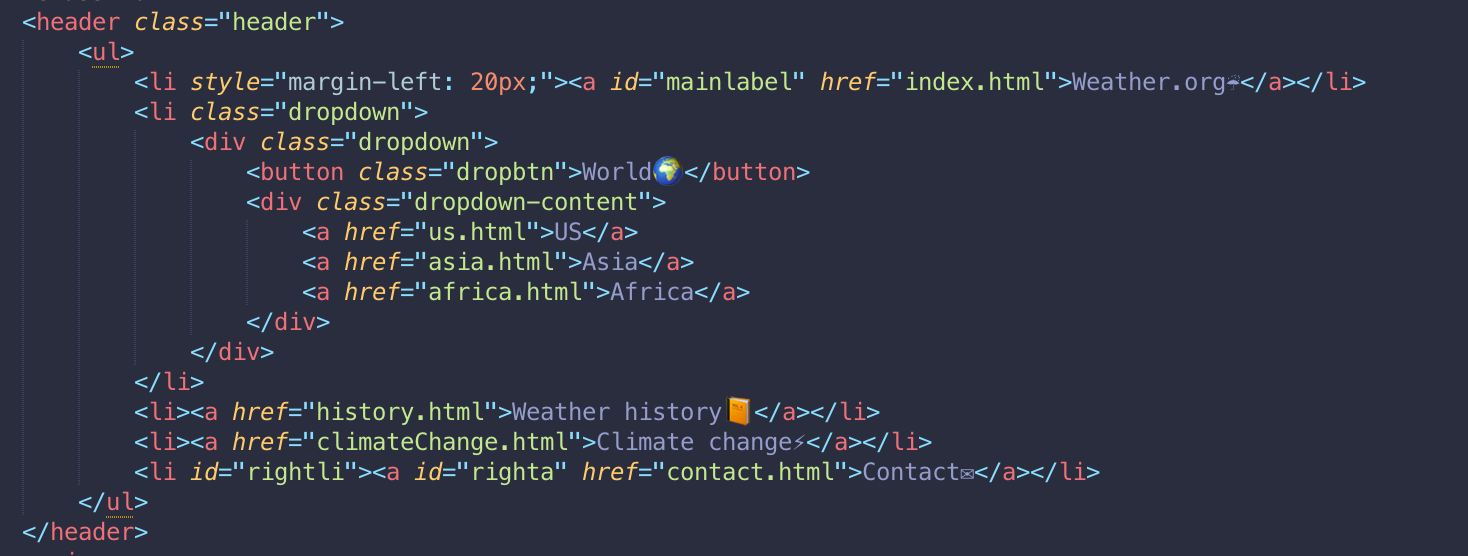
\includegraphics[scale=0.55]{fig/panel_navigatiob.png}
    \caption{Реализация панели навигации}
    \label{fig:fig1}
\end{figure}



\subsection{Домашняя страница}
Домашняя страница представляет из себя: панель навигации, \textit{gif}-файл с картой мира, список ссылок на метеорологические данные разных стран. Код разметки домашней страницы размещается в файле \textit{index.html} корневой директории проекта и приведён ниже.



\section[Руководство пользователя]{РУКОВОДСТВО ПОЛЬЗОВАТЕЛЯ}

Главная страница предоставлена на рисунке~\ref{fig:fig3}. С нее пользователь может перемещаться по страницам веб-сайта посредством Панели Навигации -- рисунок~\ref{fig:fig4}. На ней так же представлен список ссылок на метеорологические данные разных стран.

\begin{figure}[htbp]
    \centering
    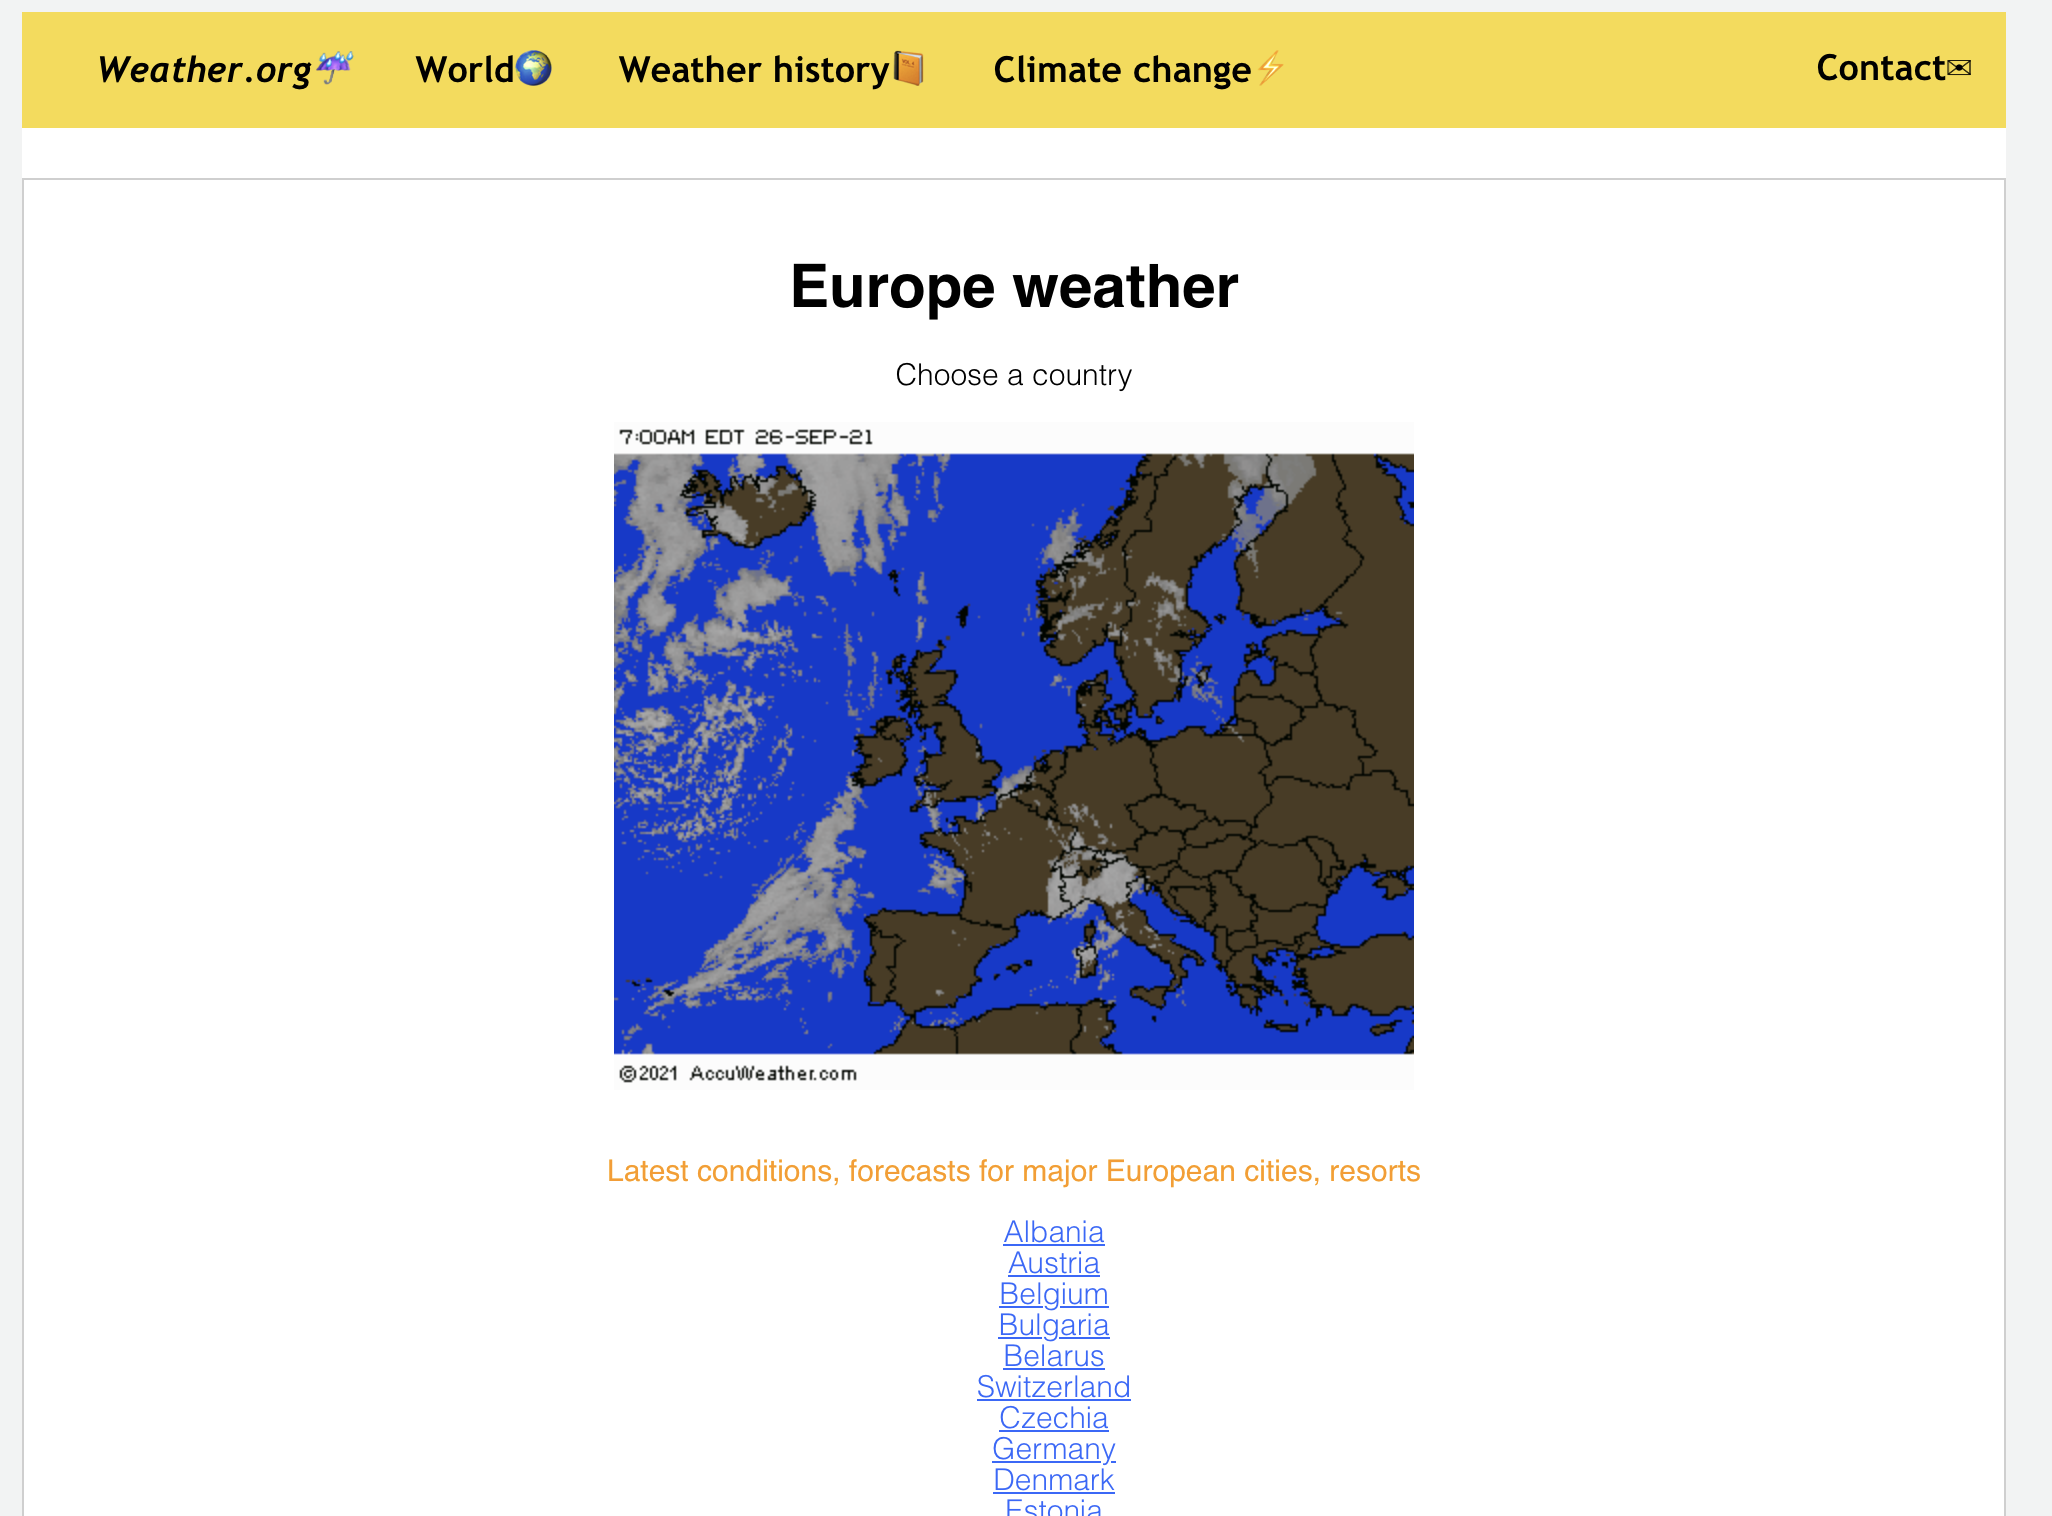
\includegraphics[scale=0.4]{fig/index.png}
    \caption{Главная страница}
    \label{fig:fig3}
\end{figure}

\begin{figure}[htbp]
    \centering
    
\includegraphics[scale=0.4]{fig/panel.png}
    \caption{Панель навигации}
    \label{fig:fig4}
\end{figure}


%%%%%%%%%%%%%%%%/ page %%%%%%%%%%%%%%%%/

Страница \textit{Weather history} cодержит историческую справку о погодных условиях. Это показано на рисунке~\ref{fig:fig5}. C этой страницы посредством Панели Навигации пользователь может переместиться на любую другую страницу, а так же на\textit{ index.html}.

\begin{figure}[htbp]
    \centering
    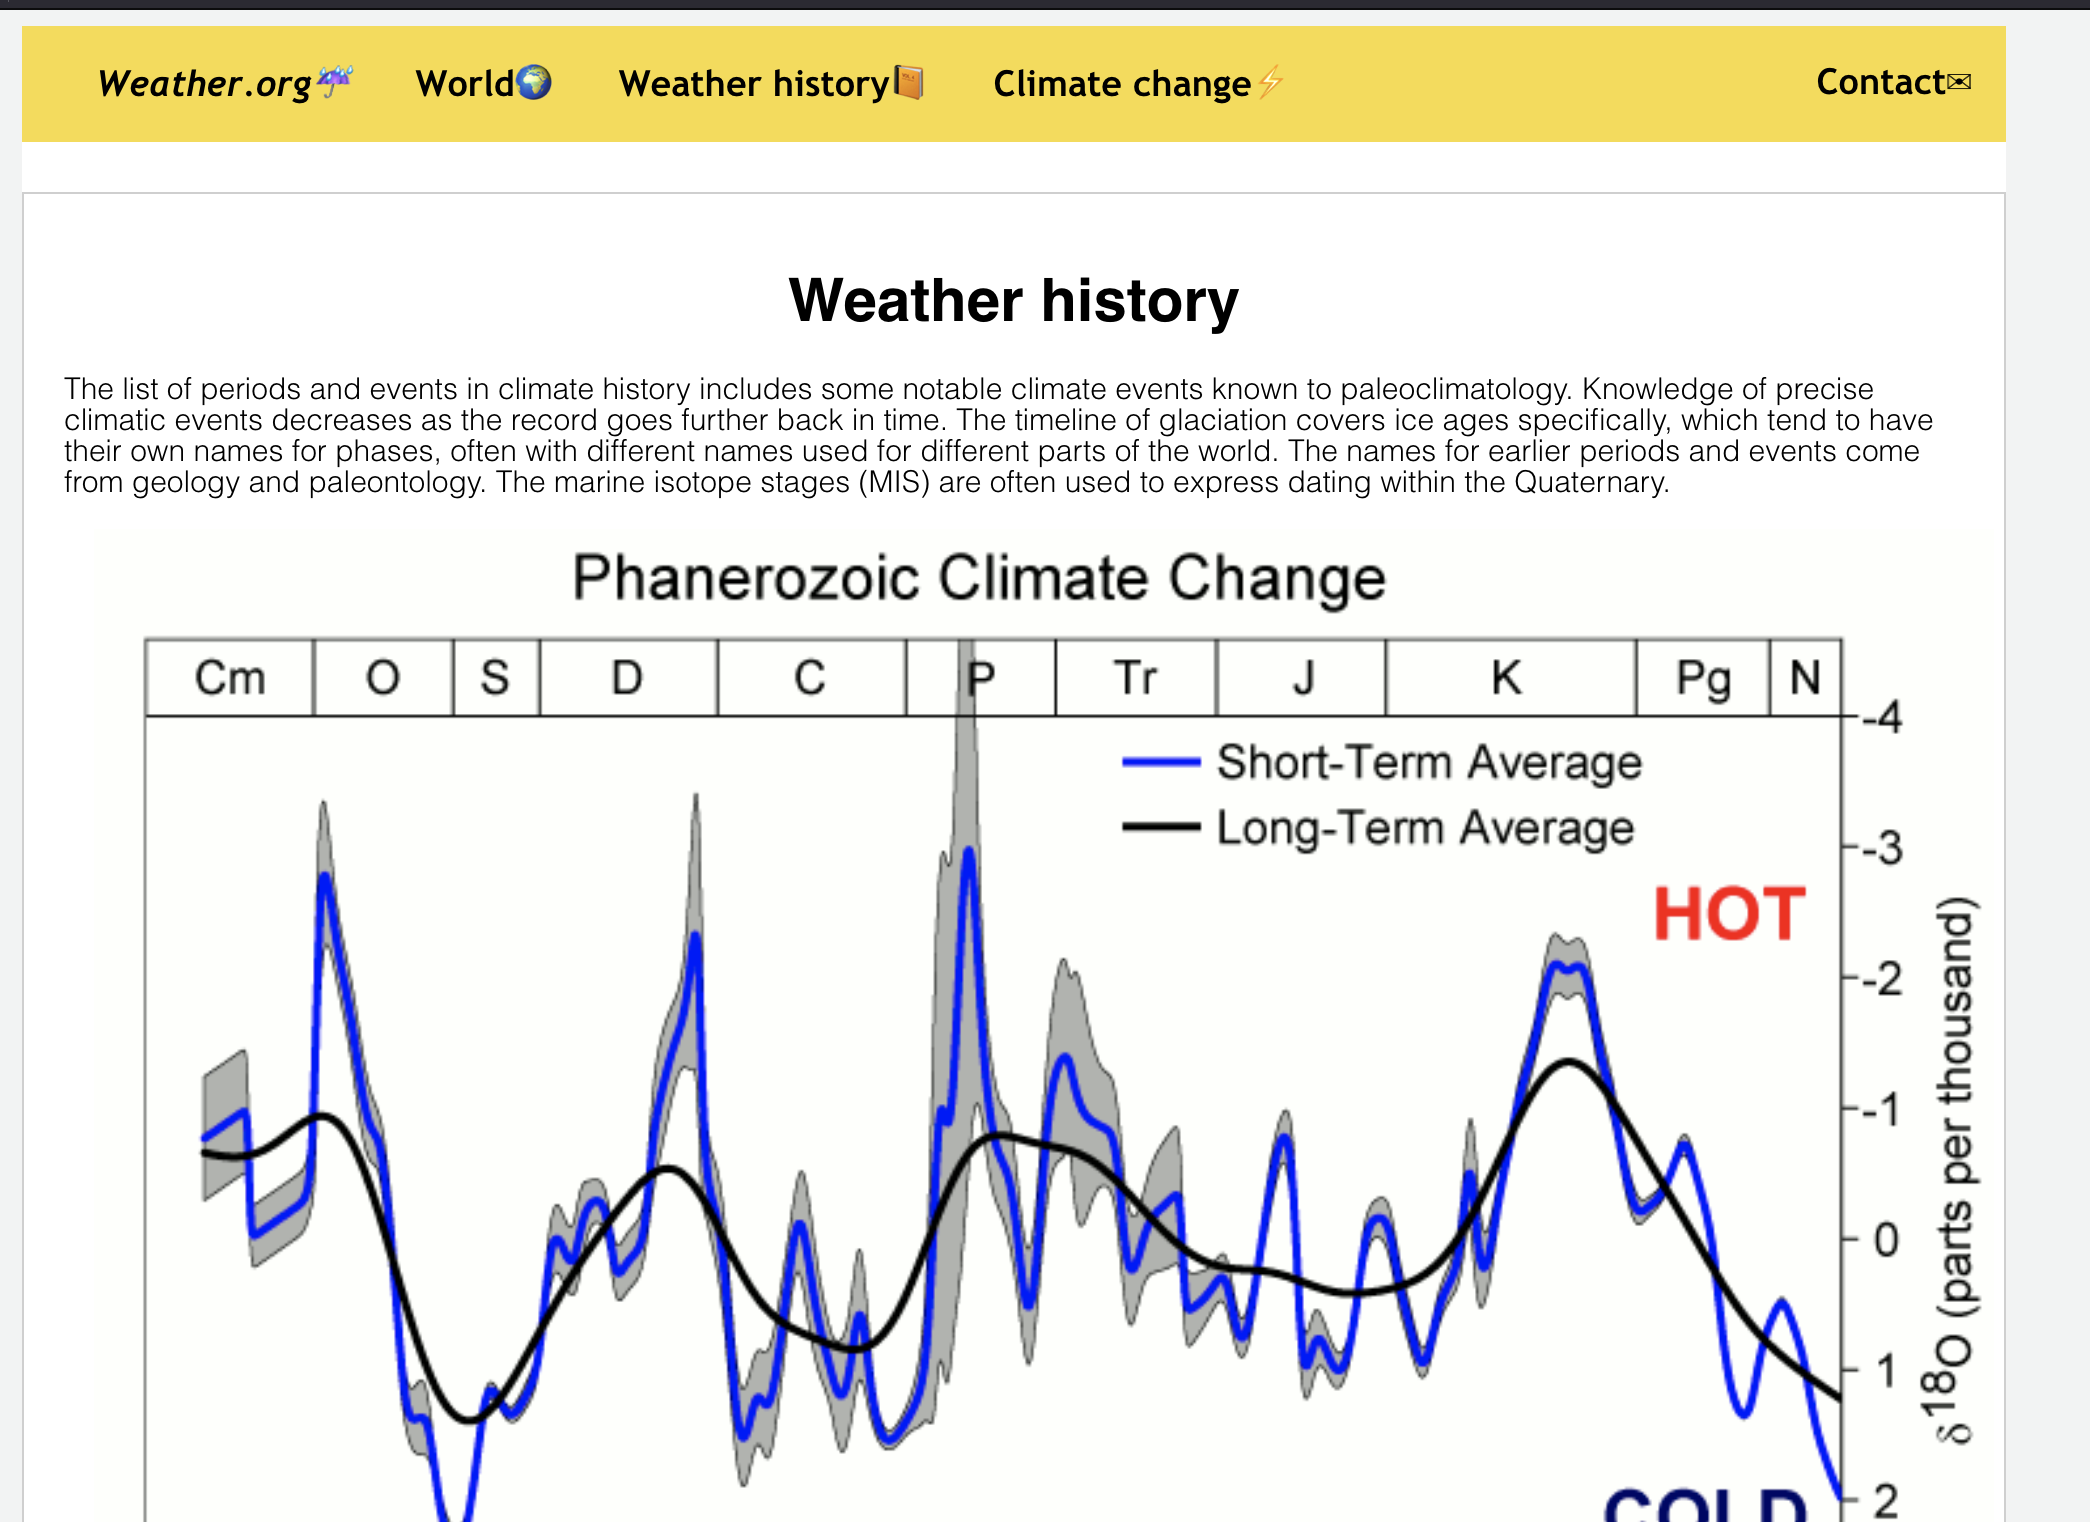
\includegraphics[scale=0.3]{fig/history.png}
    \caption{Страница \textit{Weather history}}
    \label{fig:fig5}
\end{figure}


%%%%%%%%%%%%%%%%/ page %%%%%%%%%%%%%%%%/

Страница \textit{Climate change} cодержит информационную справку об изменении климата и прогнозах на будущее. Это показано на рисунке~\ref{fig:fig6}. C этой страницы посредством Панели Навигации пользователь может переместиться на любую другую страницу, а так же на\textit{ index.html}. На данной странице содержится подробная информация об изменении климата и последние данные на сегодняшний день.

\begin{figure}[htbp!]
    \centering
    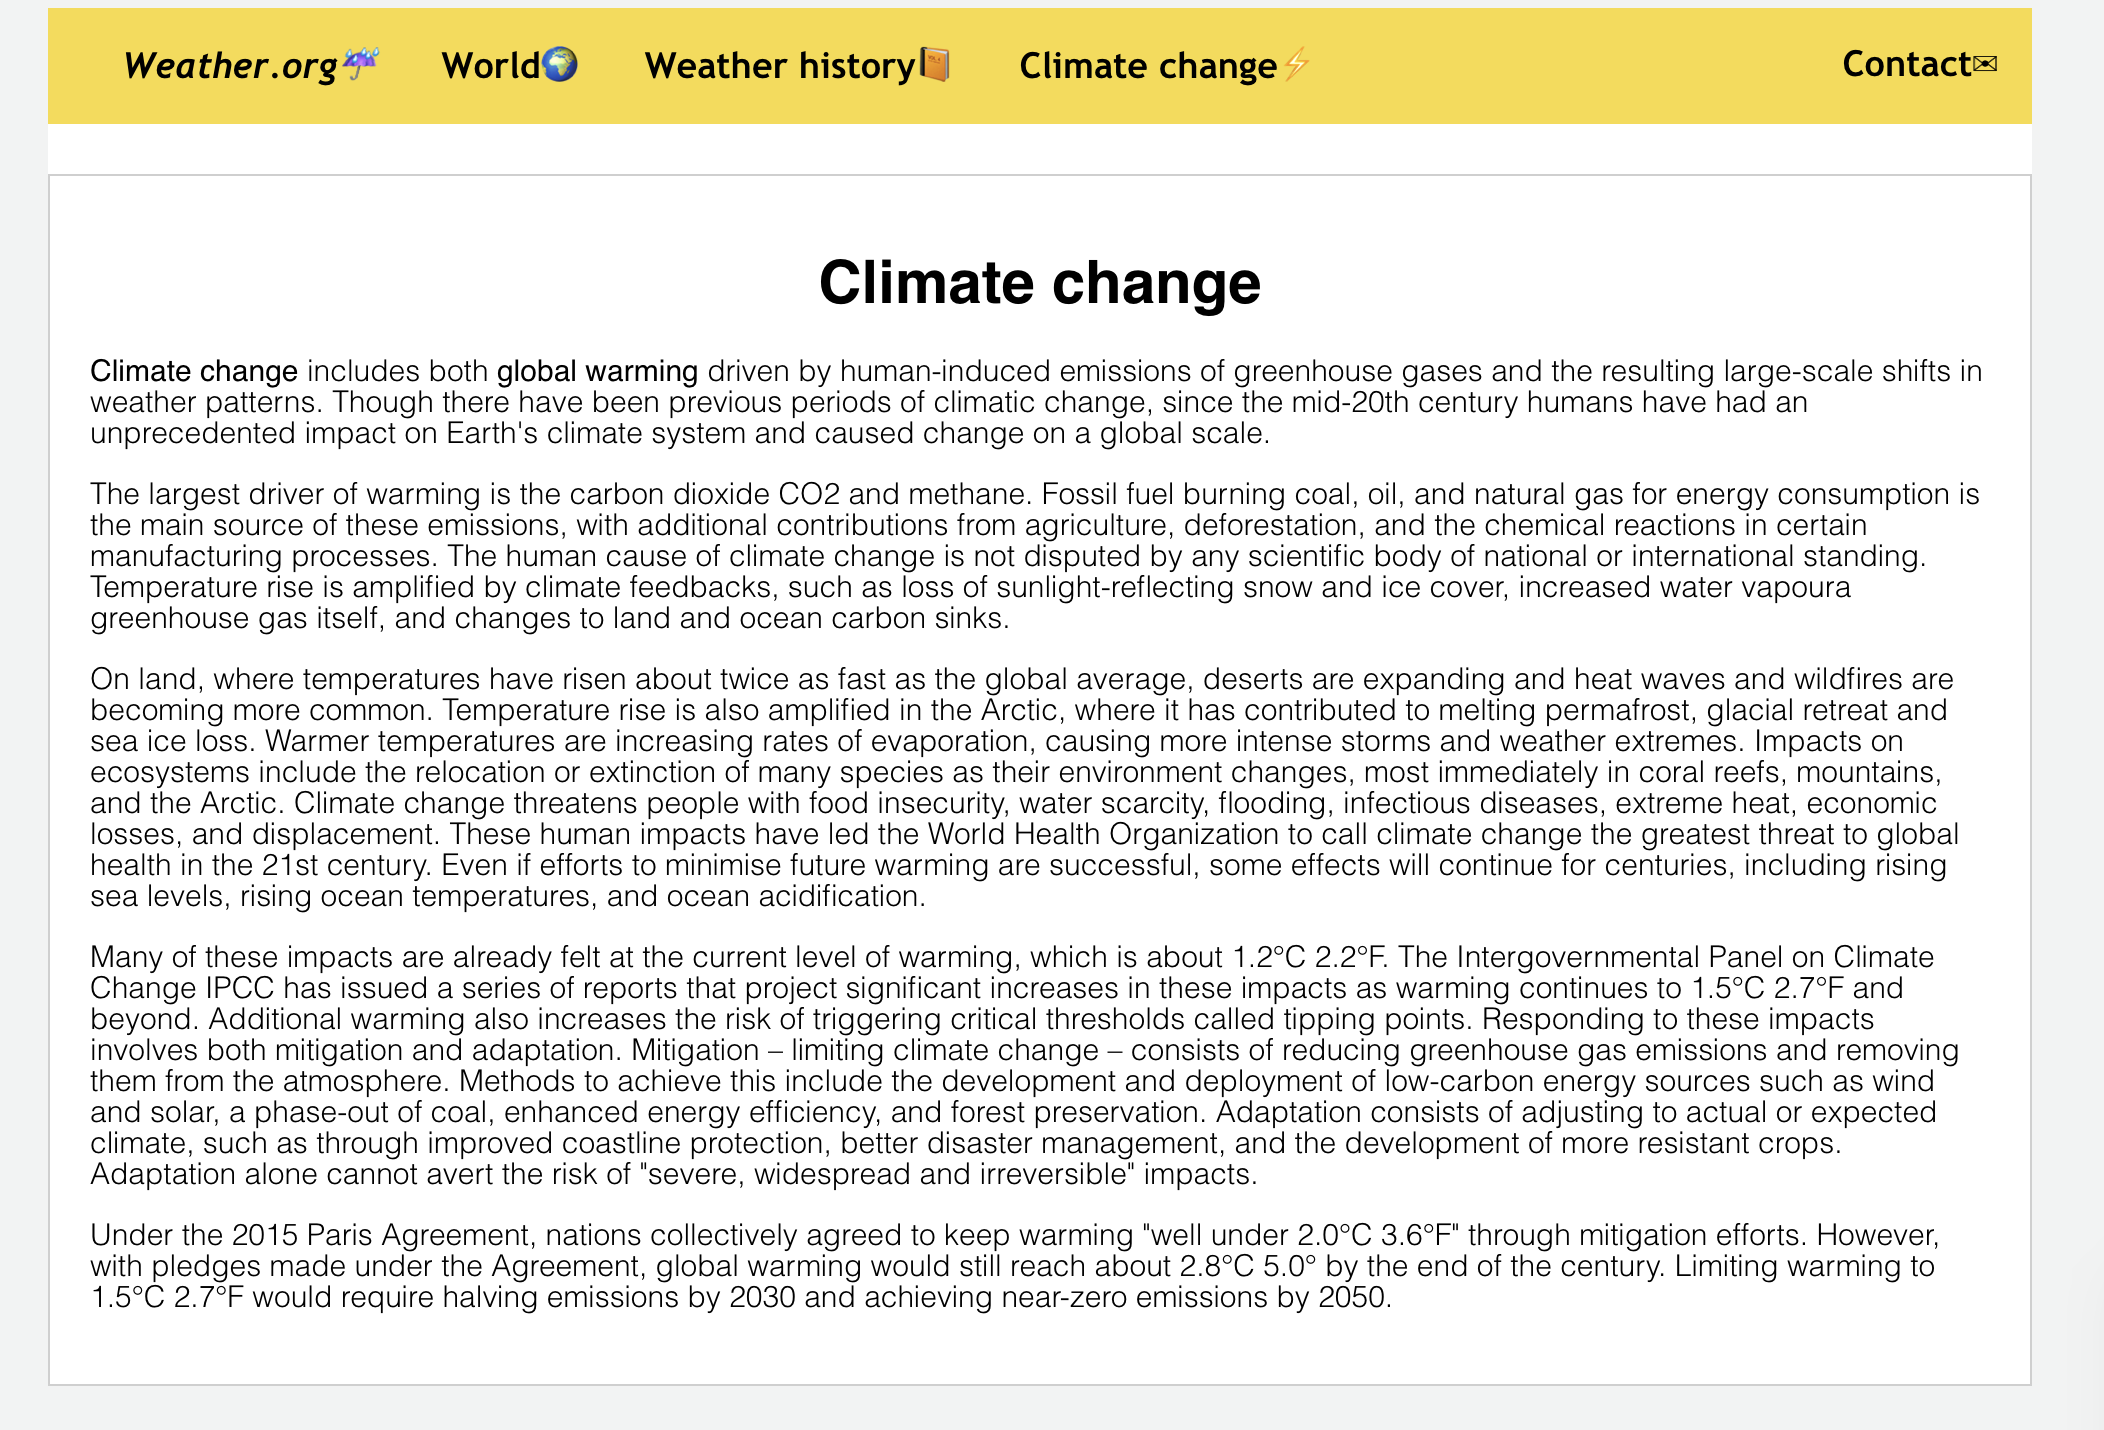
\includegraphics[scale=0.4]{fig/change.png}
    \caption{Страница \textit{Climate change}}
    \label{fig:fig6}
\end{figure}

\clearpage

%%%%%%%%%%%%%%%%/ page %%%%%%%%%%%%%%%%/

Страница \textit{US weather} cодержит информационную справку о климате США. Это представлено на рисунке~\ref{fig:fig7}. C этой страницы посредством Панели Навигации пользователь может переместиться на любую другую страницу, а так же на\textit{ index.html}. Здесь пользователь может видеть невероятную информацию о метеорологических условиях всех Соединенных Штатов Америке в формате карты.

\begin{figure}[htbp]
    \centering
    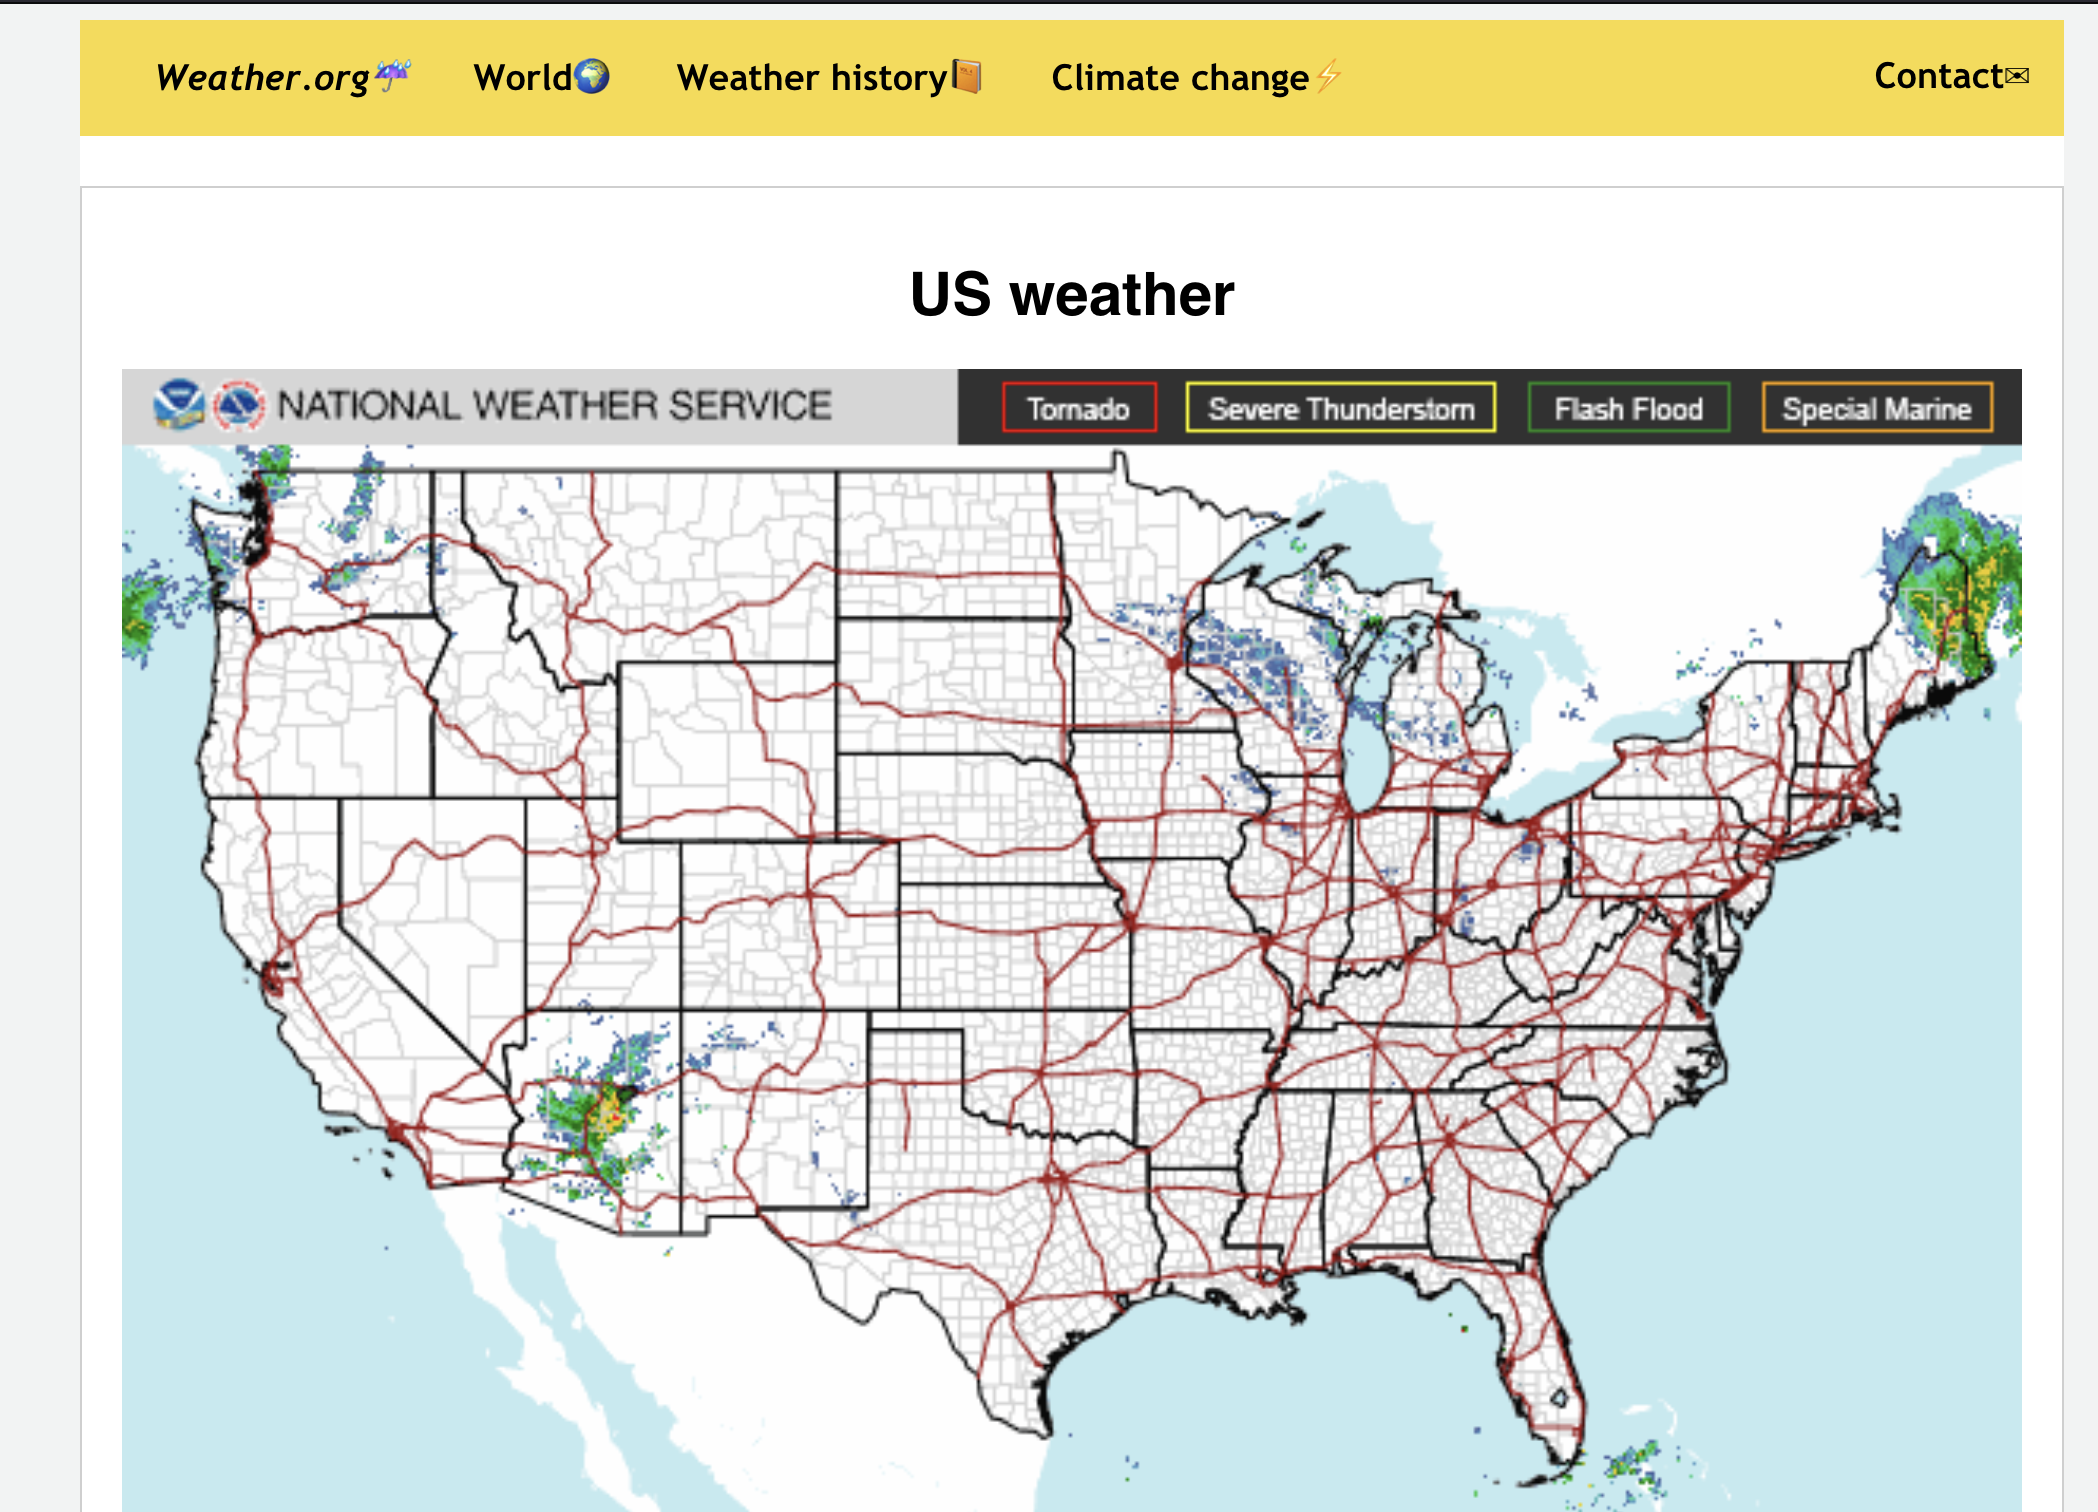
\includegraphics[scale=0.4]{fig/w_usa.png}
    \caption{Страница \textit{US weather}}
    \label{fig:fig7}
\end{figure}

%%%%%%%%%%%%%%%%/ page %%%%%%%%%%%%%%%%/
Страница \textit{Asia weather} (рисунок~\ref{fig:fig8}) cодержит информационную справку о климате Азии ознакомительные картинки. C этой страницы посредством Панели Навигации пользователь может переместиться на любую другую страницу, а так же на\textit{ index.html}.

\begin{figure}[htbp]
    \centering
    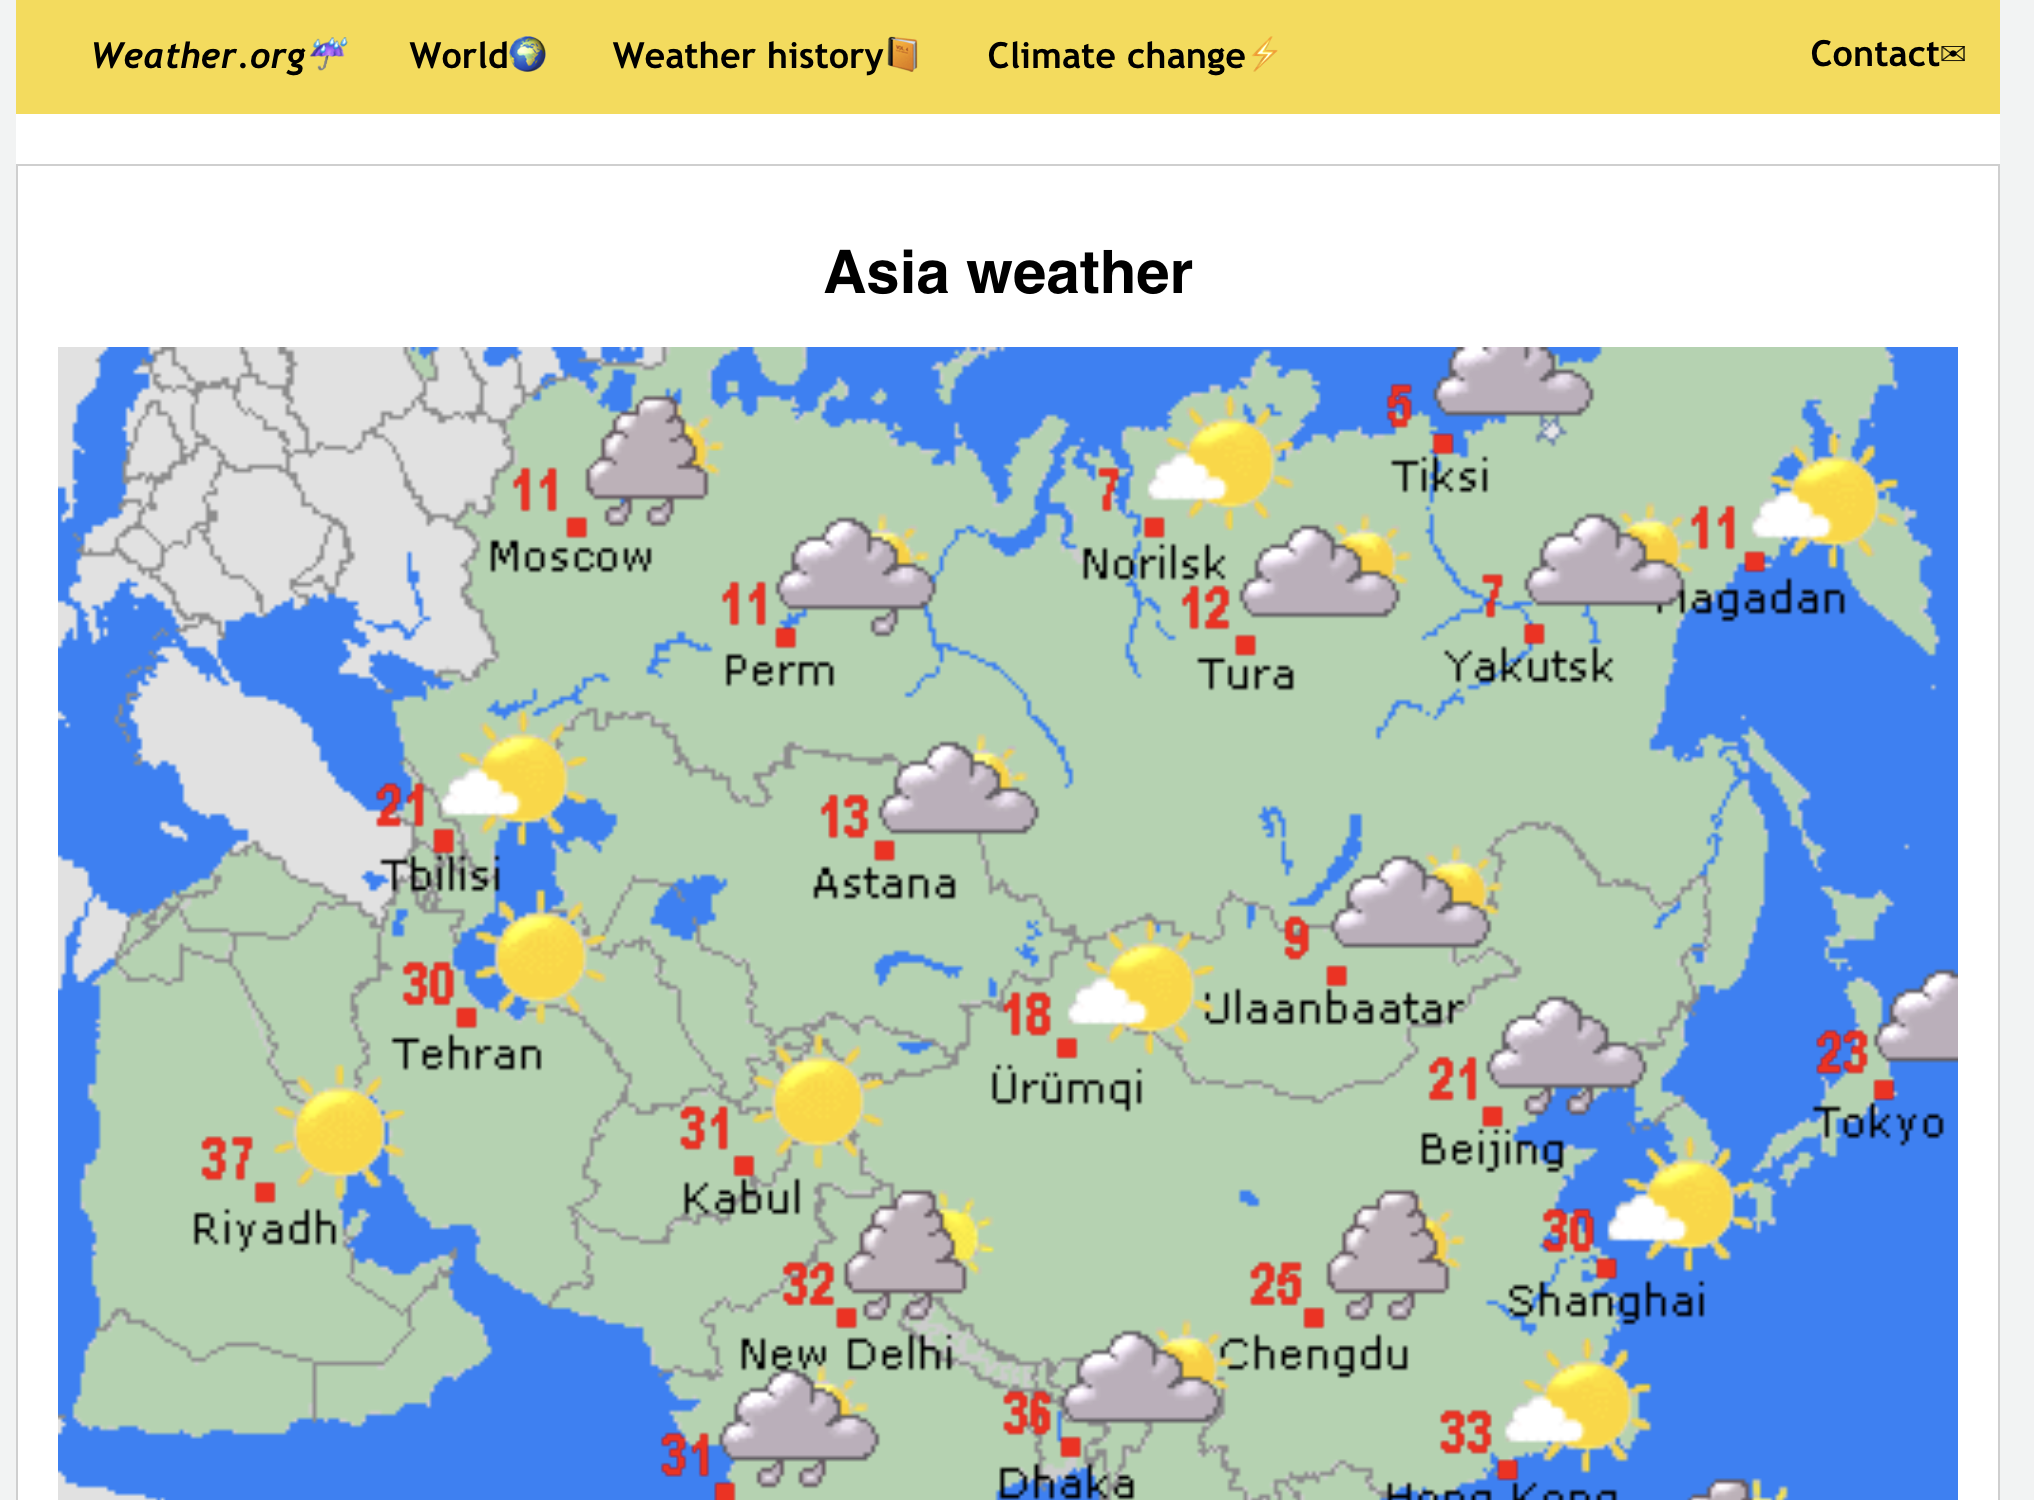
\includegraphics[scale=0.4]{fig/w_asia.png}
    \caption{Страница \textit{Asia weather}}
    \label{fig:fig8}
\end{figure}


%%%%%%%%%%%%%%%%/ page %%%%%%%%%%%%%%%%/
Страница \textit{Africa weather} (рисунок~\ref{fig:fig9}) cодержит информационную справку о климате Азии ознакомительные картинки. C этой страницы посредством Панели Навигации пользователь может переместиться на любую другую страницу, а так же на\textit{ index.html}.

\begin{figure}[htbp]
    \centering
    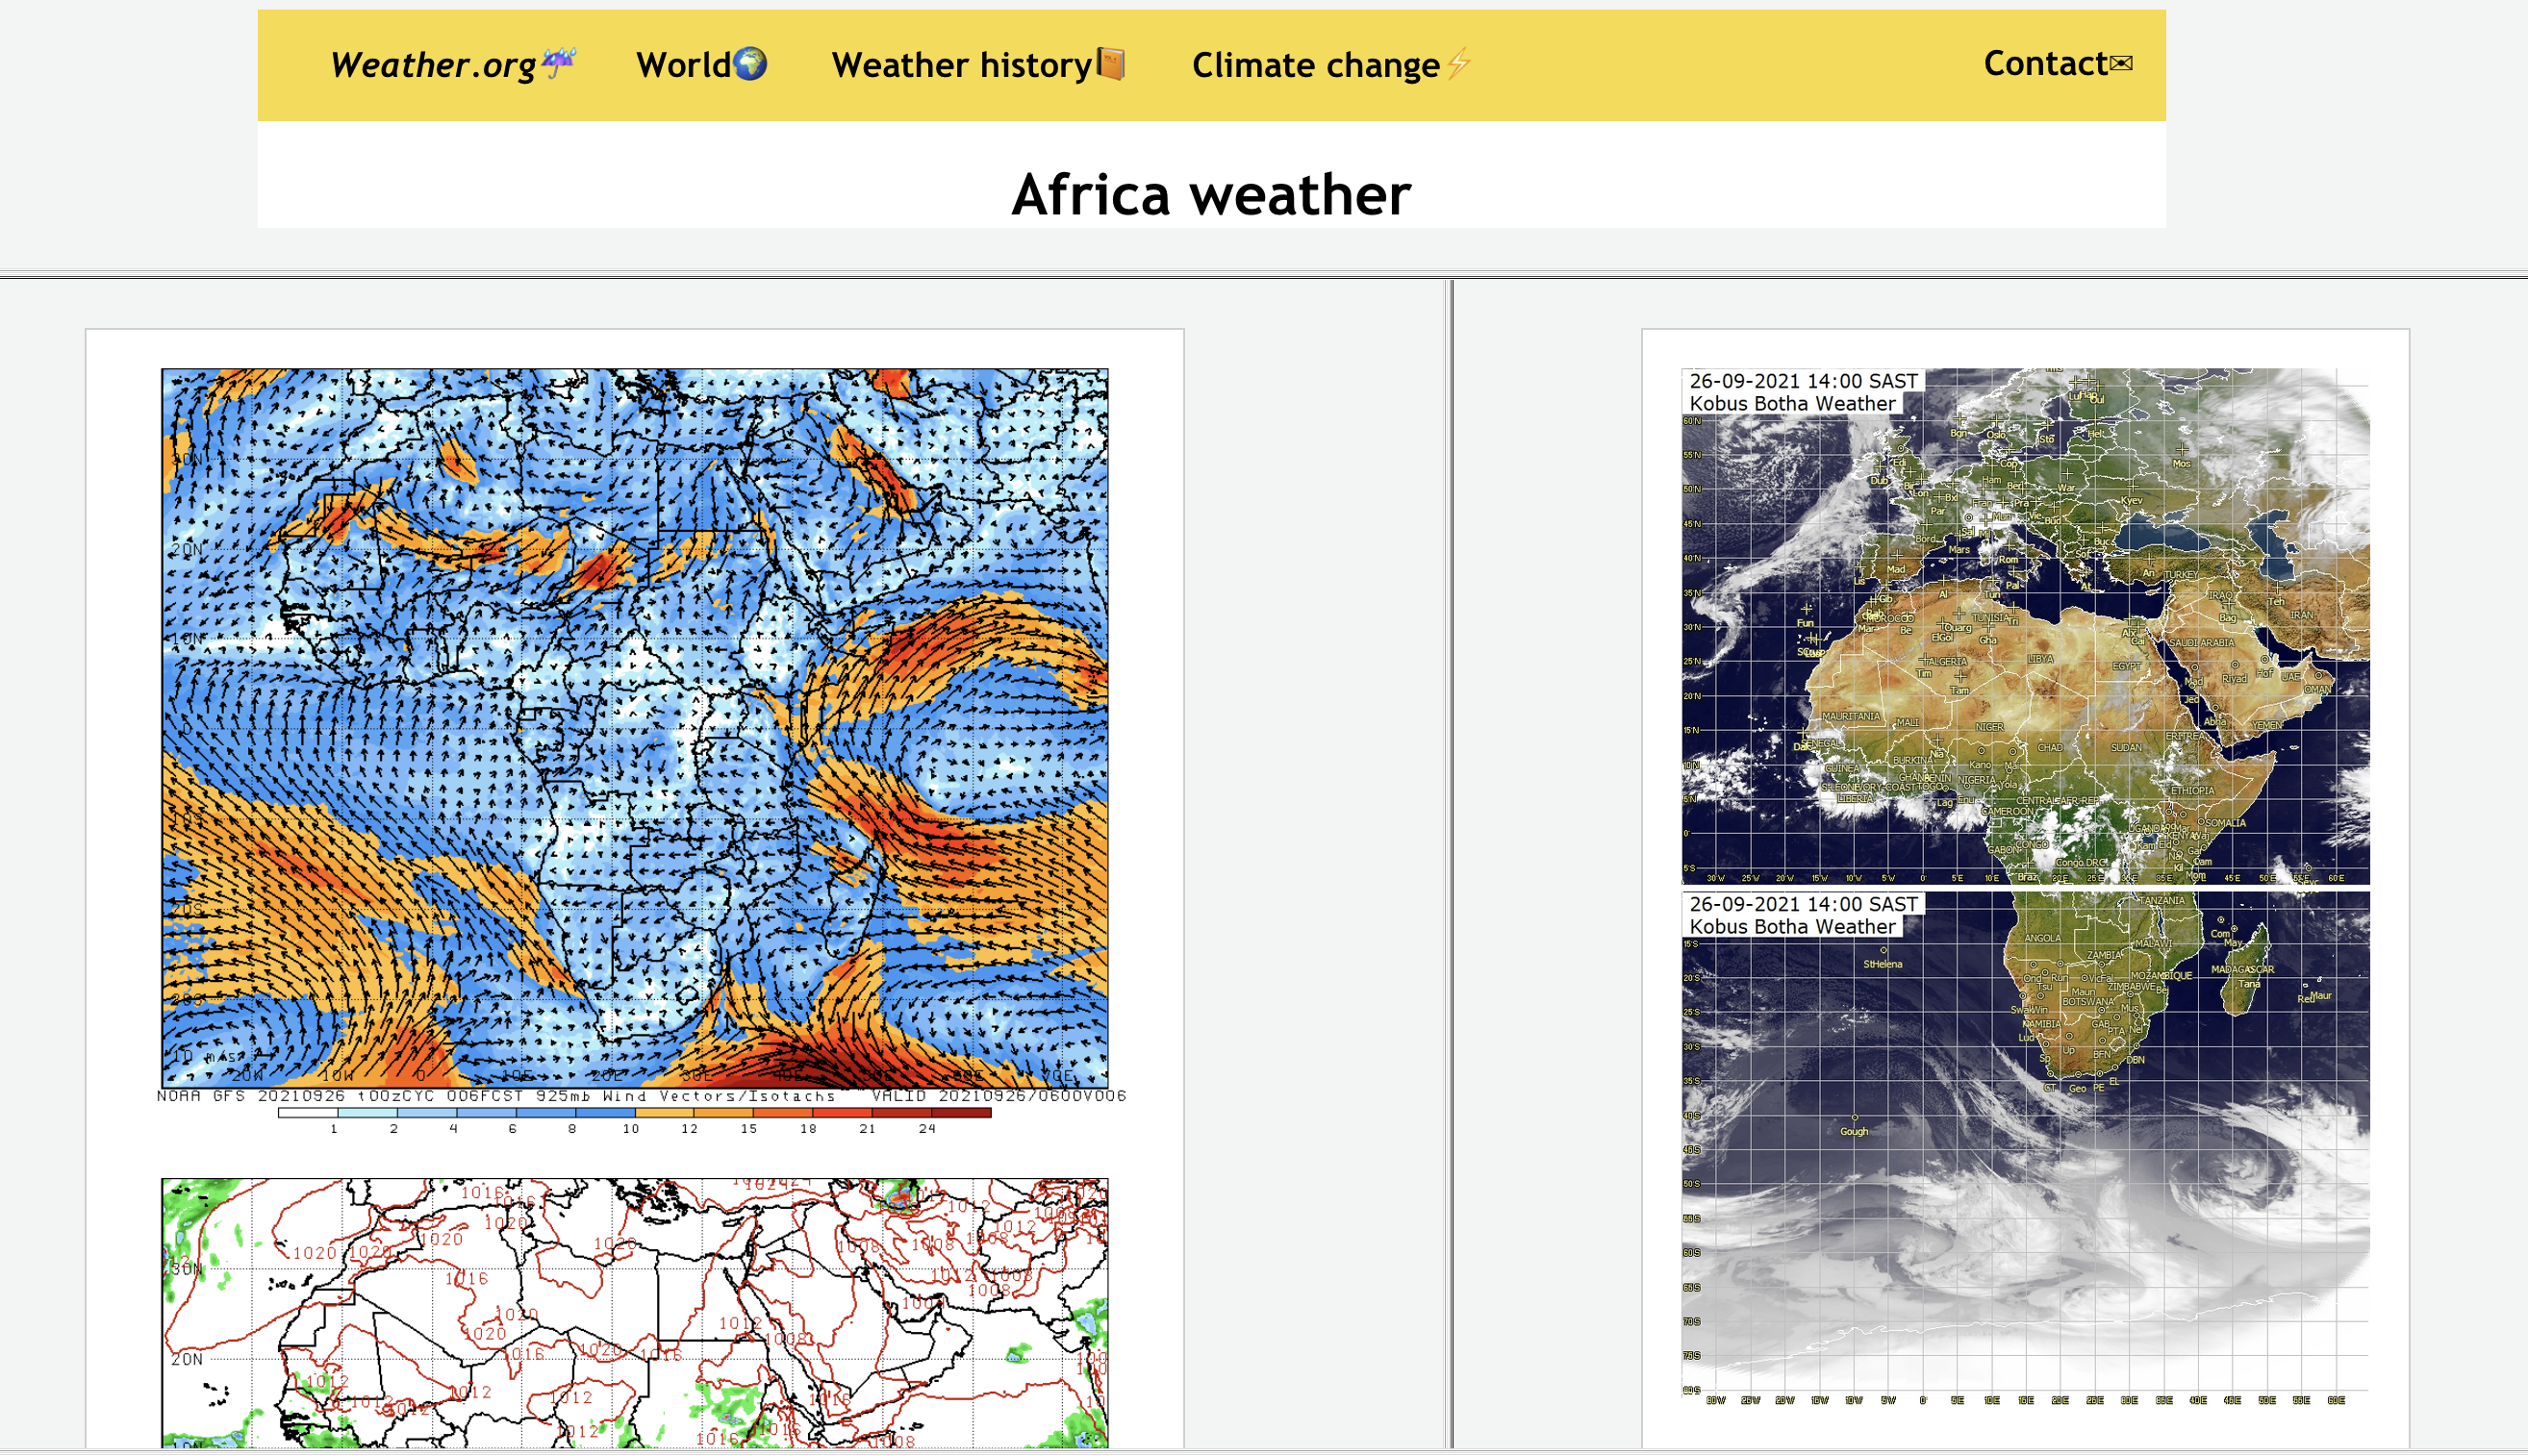
\includegraphics[scale=0.4]{fig/w_africa.png}
    \caption{Страница \textit{Africa weather}}
    \label{fig:fig9}
\end{figure}

\clearpage
%%%%%%%%%%%%%%%%/ page %%%%%%%%%%%%%%%%/
Страница \textit{Contact} содержит форму обратной связи -- это видно на рисунке~\ref{fig:fig10}. Данная форма предназначена для получения зачета по ТИП с вероятностью 110\%. C этой страницы посредством Панели Навигации пользователь может переместиться на любую другую страницу, а так же на\textit{index.html}.

\begin{figure}[htbp]
    \centering
    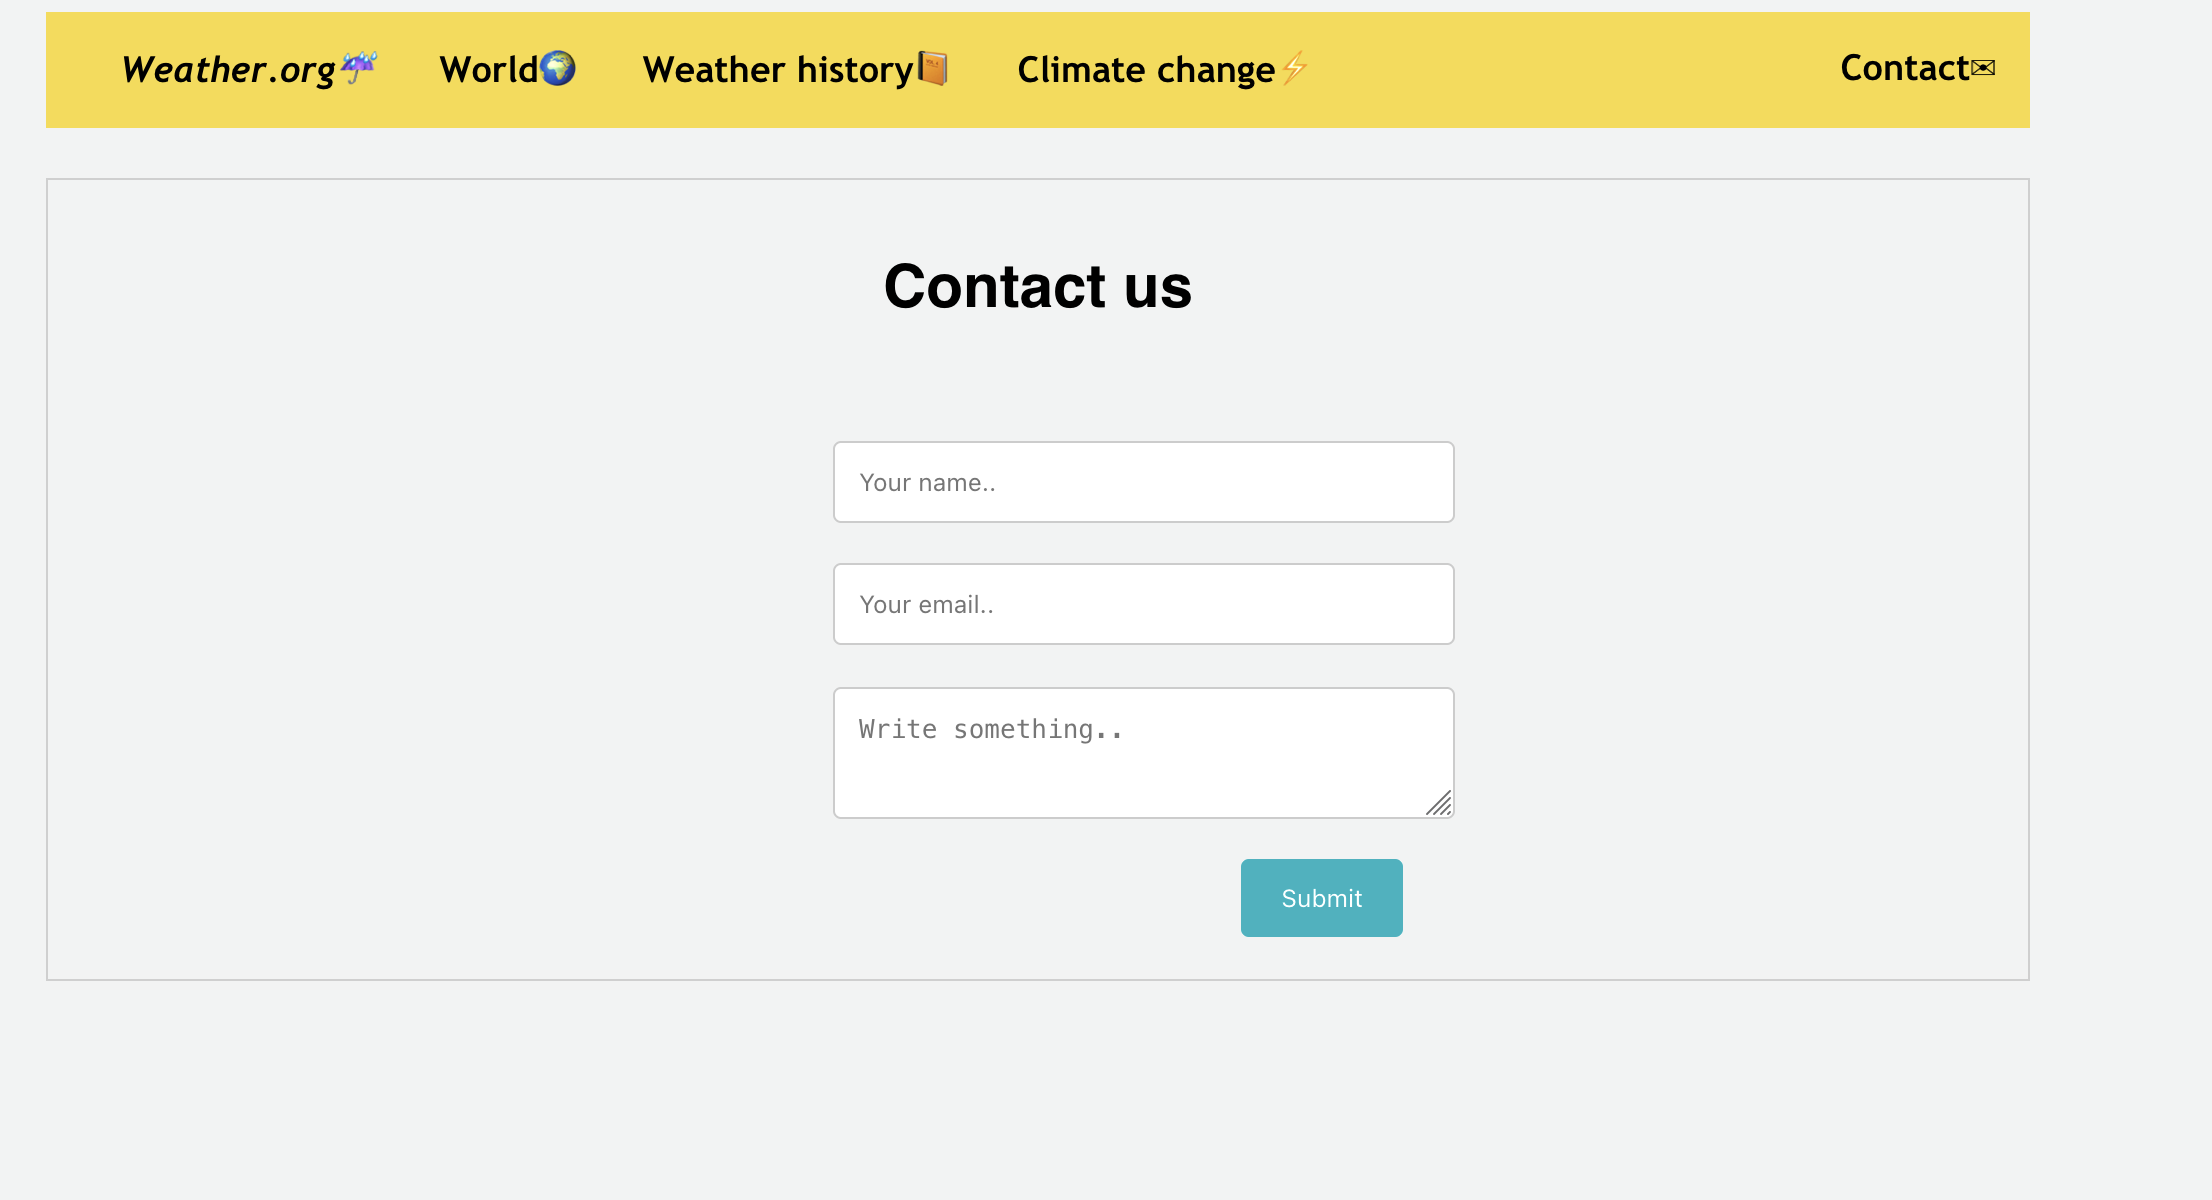
\includegraphics[scale=0.4]{fig/contact.png}
    \caption{Страница \textit{Contact}}
    \label{fig:fig10}
\end{figure}



%\section*{ЗАКЛЮЧЕНИЕ}

В ходе проведения лабораторной работы нами было установлено\dots,
дальше следует точная копия целей работы, оформленная на этот раз в 
виде обычного текста.

\newpage

  % Заключение
\addcontentsline{toc}{section}{Заключение}
\section*{ЗАКЛЮЧЕНИЕ}

В ходе выполнения лабораторной работы был разработан сайт на тему «Погода на планете». Разработка велась посредством языка разметки \textit{HTML} и его возможностей, так же были использованы каскадные таблицы стилей для улучшение визуального вида страниц сайта.


%\addcontentsline{toc}{section}{Список использованных источников}
%\begin{thebibliography}{2}
%
%    \bibitem{1} Алексеев В. Ф. \emph{Основы информационных технологий. Лабораторный практикум : пособие} / В. Ф. Алексеев, Т. В. Русак, Г. А. Пискун. - Минск : БГУИР, 2017. - 104 с. : ил.
%
%    \bibitem{2}  Фримен Эл.  \emph{Изучаем HTML, XHTML и CSS} / Фримен Эл., Фримен Эр. - Санкт-Петербург : Питер, 2013. - 656 с.
%\end{thebibliography}

%\renewcommand{\thefigure}{\Asbuk{section}.\arabic{figure}}
\renewcommand{\thetable}{\Asbuk{section}.\arabic{table}}
\renewcommand{\thelstlisting}{\Asbuk{section}.\arabic{lstlisting}}

\chead{\vspace{1ex}Продолжение приложения А}
\pagestyle{fancy}
\thispagestyle{plain}

\section*{ПРИЛОЖЕНИЕ A\\(справочное)\\Листинг Кода Страниц}

\setcounter{section}{1}
\setcounter{figure}{0}
\setcounter{table}{0}
\setcounter{lstlisting}{0}

В редких случаях бывает удобно выделять объемные рисунки и таблицы, а также листиниги в приложения:

\begin{lstlisting}[language=HTML,caption=Исходный код страницы Index]
    <!DOCTYPE html>
    <html lang="en">
    <head>
    <meta charset="utf-8">
    <title>Weather.org</title>
    <link rel="stylesheet" href="style.css">
    </head>
    <body>
    <div class="all">
    <header class="header">
    <ul>
    <li style="margin-left: 20px;"><a id="mainlabel" href="index.html">Weather.org</a></li>
    <li class="dropdown">
    <div class="dropdown">
    <button class="dropbtn">World</button>
    <div class="dropdown-content">
    <a href="us.html">US</a>
    <a href="asia.html">Asia</a>
    <a href="africa.html">Africa</a>
    </div>
    </div>
    </li>
    <li><a href="history.html">Weather history</a></li>
    <li><a href="climateChange.html"></a></li>
    <li id="rightli"><a id="righta" href="contact.html">Contact</a></li>
    </ul>
    </header>
    <main>
    <div class="content">
    <center>
    <h1>Europe weather</h1>
    <p>Choose a country</p>
    <div style="margin-bottom: 30px;">
    <img src="images/europe.gif" alt="europe" usemap=#navigation>
    <map name=navigation>
    <area shape=circle coords="354,164,13"
    href=belarus.html alt="Belarus">
    <area shape=circle coords="300,176,20"
    href=poland.html alt="Poland">
    <area shape=circle coords="245,180,10"
    href=https://www.accuweather.com/en/browse-locations/eur/de alt="Germany">
    <area shape=rect coords="333,187,394,200"
    href=https://www.accuweather.com/en/browse-locations/eur/ua" alt="Ukraine">
    <area shape=circle coords="173,172,18"
    href=https://www.accuweather.com/en/browse-locations/eur/gb alt="Great Britan">
    <area shape=circle coords="197,221,22"
    href=https://www.accuweather.com/en/browse-locations/eur/fr alt="France">
    </map>
    </div>
    <strong><span style="color: #ff9900; text-align: left;">Latest conditions, forecasts for major European cities, resorts</span></strong>
    <ul class="listlink">
    <li>
    <div>
    <a  href="https://www.accuweather.com/en/browse-locations/eur/al">Albania</a>
    </div>
    </li>
    <li>
    <div>
    <a href="https://www.accuweather.com/en/browse-locations/eur/at" >Austria</a>
    </div>
    </li>
    <li>
    <div>
    <a href="https://www.accuweather.com/en/browse-locations/eur/be">Belgium</a>
    </div>
    </li>
    <li>
    <div>
    <a href="https://www.accuweather.com/en/browse-locations/eur/bg">Bulgaria</a>
    </div>
    </li>
    <li>
    <div>
    <a href="https://www.accuweather.com/en/browse-locations/eur/by">Belarus</a>
    </div>
    </li>
    <li>
    <div>
    <a href="https://www.accuweather.com/en/browse-locations/eur/ch">Switzerland</a>
    </div>
    </li>
    <li>
    <div>
    <a href="https://www.accuweather.com/en/browse-locations/eur/cz">Czechia</a>
    </div>
    </li>
    <li>
    <div>
    <a href="https://www.accuweather.com/en/browse-locations/eur/de">Germany</a>
    </div>
    </li>
    <li>
    <div>
    <a href="https://www.accuweather.com/en/browse-locations/eur/dk">Denmark</a>
    </div>
    </li>
    <li>
    <div>
    <a href="https://www.accuweather.com/en/browse-locations/eur/ee">Estonia</a>
    </div>
    </li>
    <li>
    <div>
    <a href="https://www.accuweather.com/en/browse-locations/eur/es">Spain</a>
    </div>
    </li>
    <li>
    <div>
    <a href="https://www.accuweather.com/en/browse-locations/eur/fi">Finland</a>
    </div>
    </li>
    <li>
    <div>
    <a href="https://www.accuweather.com/en/browse-locations/eur/fr">France</a>
    </div>
    </li>
    <li>
    <div>
    <a href="https://www.accuweather.com/en/browse-locations/eur/gb">United Kingdom</a>
    </div>
    </li>
    <li>
    <div>
    <a href="https://www.accuweather.com/en/browse-locations/eur/gr">Greece</a>
    </div>
    </li>
    <li>
    <div>
    <a href="https://www.accuweather.com/en/browse-locations/eur/hr">Croatia</a>
    </div>
    </li>
    <li>
    <div>
    <a href="https://www.accuweather.com/en/browse-locations/eur/hu">Hungary</a>
    </div>
    </li>
    <li>
    <div>
    <a href="https://www.accuweather.com/en/browse-locations/eur/ie">Ireland</a>
    </div>
    </li>
    <li>
    <div>
    <a href="https://www.accuweather.com/en/browse-locations/eur/it">Italy</a>
    </div>
    </li>
    <li>
    <div>
    <a href="https://www.accuweather.com/en/browse-locations/eur/lt">Lithuania</a>
    </div>
    </li>
    <li>
    <div>
    <a href="https://www.accuweather.com/en/browse-locations/eur/lv">Latvia</a>
    </div>
    </li>
    <li>
    <div>
    <a href="https://www.accuweather.com/en/browse-locations/eur/md">Moldova</a>
    </div>
    </li>
    <li>
    <div>
    <a href="https://www.accuweather.com/en/browse-locations/eur/nl">Netherlands</a>
    </div>
    </li>
    <li>
    <div>
    <a href="https://www.accuweather.com/en/browse-locations/eur/no">Norway</a>
    </div>
    </li>
    <li>
    <div>
    <a href="https://www.accuweather.com/en/browse-locations/eur/pl">Poland</a>
    </div>
    </li>
    <li>
    <div>
    <a href="https://www.accuweather.com/en/browse-locations/eur/pt">Portugal</a>
    </div>
    </li>
    <li>
    <div>
    <a href="https://www.accuweather.com/en/browse-locations/eur/ro">Romania</a>
    </div>
    </li>
    <li >
    <div>
    <a href="https://www.accuweather.com/en/browse-locations/eur/rs">Serbia</a>
    </div>
    </li>
    <li>
    <div>
    <a href="https://www.accuweather.com/en/browse-locations/eur/ru">Russia</a>
    </div>
    </li>
    <li>
    <div>
    <a href="https://www.accuweather.com/en/browse-locations/eur/se">Sweden</a>
    </div>
    </li>
    <li>
    <div>
    <a href="https://www.accuweather.com/en/browse-locations/eur/si">Slovenia</a>
    </div>
    </li>
    <li>
    <div>
    <a href="https://www.accuweather.com/en/browse-locations/eur/sk">Slovakia</a>
    </div>
    </li>
    <li>
    <div>
    <a href="https://www.accuweather.com/en/browse-locations/eur/tr">Turkey</a>
    </div>
    </li>
    <li>
    <div>
    <a href="https://www.accuweather.com/en/browse-locations/eur/ua">Ukraine</a>
    </div>
    </li>
    </ul>
    </div>
    </center>
    </main>
    </div>
    </body>
    </html>
\end{lstlisting}


\begin{lstlisting}[language=HTML,caption=Исходный код страницы Africa]
   <!DOCTYPE HTML PUBLIC "-//W3C//DTD HTML 4.01 Frameset//EN" "http://www.w3.org/TR/html4/frameset.dtd">
   <html lang="en">
   <head>
   <meta charset="utf-8">
   <title>Africa</title>
   <link rel="stylesheet" href="style.css">
   </head>
   <frameset rows="32%, *" noresize scrolling="no">
   <frame src="top.html"></frame>
   <frameset cols="840, *">
   <frame src="firstframe.html">
   </frame>
   <frame src="secondframe.html"></frame>
   </frameset>
   </frameset>
   </html>
\end{lstlisting}


\begin{lstlisting}[language=HTML,caption=Исходный код страницы Asia]
    <!DOCTYPE HTML PUBLIC "-//W3C//DTD HTML 4.01 Frameset//EN" "http://www.w3.org/TR/html4/frameset.dtd">
    <html lang="en">
    <head>
    <meta charset="utf-8">
    <title>Africa</title>
    <link rel="stylesheet" href="style.css">
    </head>
    <frameset rows="32%, *" noresize scrolling="no">
    <frame src="top.html"></frame>
    <frameset cols="840, *">
    <frame src="firstframe.html">
    </frame>
    <frame src="secondframe.html"></frame>
    </frameset>
    </frameset>
    </html><!DOCTYPE html>
    <html lang="en">
    <head>
    <meta charset="utf-8">
    <title>Asia</title>
    <link rel="stylesheet" href="style.css">
    </head>
    <body>
    <div class="all">
    <header class="header">
    <ul>
    <li style="margin-left: 20px;"><a id="mainlabel" href="index.html">Weather.org☔</a></li>
    <li class="dropdown">
    <div class="dropdown">
    <button class="dropbtn">World</button>
    <div class="dropdown-content">
    <a href="us.html">US</a>
    <a href="asia.html">Asia</a>
    <a href="africa.html">Africa</a>
    </div>
    </div>
    </li>
    <li><a href="history.html">Weather history</a></li>
    <li><a href="climateChange.html">Climate change</a></li>
    <li id="rightli"><a id="righta" href="contact.html">Contact</a></li>
    </ul>
    </header>
    <main>
    <div class="content">
    <center>
    <h1>Asia weather</h1>
    <img src="images/asia1.gif" style="margin-bottom:20px; width: 100%">
    <img src="images/asia2.gif" style="margin-bottom:20px; width: 100%;">
    <img src="images/asia.jpg" style="margin-bottom:20px;width: 100%;">
    </center>
    </div>
    </main>
    </div>
    </body>
    </html>
\end{lstlisting}


\begin{lstlisting}[language=HTML,caption=Исходный код страницы Belarus]
    <!DOCTYPE html>
    <html lang="en">
    <head>
    <meta charset="utf-8">
    <title>Belarus</title>
    <link rel="stylesheet" href="style.css">
    </head>
    <body>
    <div class="all">
    <header class="header">
    <ul>
    <li style="margin-left: 20px;"><a id="mainlabel" href="index.html">Weather.org☔</a></li>
    <li class="dropdown">
    <div class="dropdown">
    <button class="dropbtn">World</button>
    <div class="dropdown-content">
    <a href="us.html">US</a>
    <a href="asia.html">Asia</a>
    <a href="africa.html">Africa</a>
    </div>
    </div>
    </li>
    <li><a href="history.html">Weather history</a></li>
    <li><a href="climateChange.html">Climate change</a></li>
    <li id="rightli"><a id="righta" href="contact.html">Contact</a></li>
    </ul>
    </header>
    <main>
    <div class="content">
    <h1>Current weather, Belarus</h1>
    <table class="weathertable">
    <tr>
    <td>
    <div class="card">
    <span class="date">26.09</span>
    <div class="icon">
    <img src="images/cloudy.png" style="width: 150px;margin-top: 40px;">
    </div>
    <span class="temperature">+13</span>
    <div class="city">Minsk</div>
    </div>
    </td>
    <td>
    <div class="card">
    <span class="date">26.09</span>
    <div class="icon">
    <img src="images/sun.png" style="width: 150px;margin-top: 40px;">
    </div>
    <span class="temperature">+15</span>
    <div class="city">Brest</div>
    </div>
    </td>
    <td>
    <div class="card">
    <span class="date">26.09</span>
    <div class="icon">
    <img src="images/sun.png" style="width: 150px;margin-top: 40px;">
    </div>
    <span class="temperature">+15</span>
    <div class="city">Grodno</div>
    </div>
    </td>
    </tr>
    <tr>
    <td>
    <div class="card">
    <span class="date">26.09</span>
    <div class="icon">
    <img src="images/cloudy.png" style="width: 150px;margin-top: 40px;">
    </div>
    <span class="temperature">+12</span>
    <div class="city">Gomel</div>
    </div>
    </td>
    <td>
    <div class="card">
    <span class="date">26.09</span>
    <div class="icon">
    <img src="images/cloudy.png" style="width: 150px;margin-top: 40px;">
    </div>
    <span class="temperature">+11</span>
    <div class="city">Vitebsk</div>
    </div>
    </td>
    <td>
    <div class="card">
    <span class="date">26.09</span>
    <div class="icon">
    <img src="images/cloudy.png" style="width: 150px;margin-top: 40px;">
    </div>
    <span class="temperature">+11</span>
    <div class="city">Mogilev</div>
    </div>
    </td>
    </tr>
    </table>
    </div>
    </main>
    </div>
    </body>
    </html>
\end{lstlisting}



\begin{lstlisting}[language=HTML,caption=Исходный код страницы Poland]
   <!DOCTYPE html>
   <html lang="en">
   <head>
   <meta charset="utf-8">
   <title>Poland</title>
   <link rel="stylesheet" href="style.css">
   </head>
   <body>
   <div class="all">
   <header class="header">
   <ul>
   <li style="margin-left: 20px;"><a id="mainlabel" href="index.html">Weather.org☔</a></li>
   <li class="dropdown">
   <div class="dropdown">
   <button class="dropbtn">World</button>
   <div class="dropdown-content">
   <a href="us.html">US</a>
   <a href="asia.html">Asia</a>
   <a href="africa.html">Africa</a>
   </div>
   </div>
   </li>
   <li><a href="history.html">Weather history</a></li>
   <li><a href="climateChange.html">Climate change</a></li>
   <li id="rightli"><a id="righta" href="contact.html">Contact</a></li>
   </ul>
   </header>
   <main>
   <div class="content">
   <h1>Current weather, Poland</h1>
   <table class="weathertable">
   <tr>
   <td>
   <div class="card">
   <span class="date">26.09</span>
   <div class="icon">
   <img src="images/sun.png" style="width: 150px;margin-top: 40px;">
   </div>
   <span class="temperature">+19</span>
   <div class="city">Krakow</div>
   </div>
   </td>
   <td>
   <div class="card">
   <span class="date">26.09</span>
   <div class="icon">
   <img src="images/sun.png" style="width: 150px;margin-top: 40px;">
   </div>
   <span class="temperature">+16</span>
   <div class="city">Bialystok</div>
   </div>
   </td>
   <td>
   <div class="card">
   <span class="date">26.09</span>
   <div class="icon">
   <img src="images/cloudy.png" style="width: 150px;margin-top: 40px;">
   </div>
   <span class="temperature">+18</span>
   <div class="city">Warsaw</div>
   </div>
   </td>
   </tr>
   <tr>
   <td>
   <div class="card">
   <span class="date">26.09</span>
   <div class="icon">
   <img src="images/cloud.png" style="width: 150px;margin-top: 40px;">
   </div>
   <span class="temperature">+17</span>
   <div class="city">Zakopane</div>
   </div>
   </td>
   <td>
   <div class="card">
   <span class="date">26.09</span>
   <div class="icon">
   <img src="images/sun.png" style="width: 150px;margin-top: 40px;">
   </div>
   <span class="temperature">+14</span>
   <div class="city">Gdansk</div>
   </div>
   </td>
   <td>
   <div class="card">
   <span class="date">26.09</span>
   <div class="icon">
   <img src="images/sun.png" style="width: 150px;margin-top: 40px;">
   </div>
   <span class="temperature">+16</span>
   <div class="city">Lublin</div>
   </div>
   </td>
   </tr>
   <tr>
   <td>
   <div class="card">
   <span class="date">26.09</span>
   <div class="icon">
   <img src="images/sun.png" style="width: 150px;margin-top: 40px;">
   </div>
   <span class="temperature">+17</span>
   <div class="city">Katowice</div>
   </div>
   </td>
   <td>
   <div class="card">
   <span class="date">26.09</span>
   <div class="icon">
   <img src="images/sun.png" style="width: 150px;margin-top: 40px;">
   </div>
   <span class="temperature">+17</span>
   <div class="city">Lodz</div>
   </div>
   </td>
   <td>
   <div class="card">
   <span class="date">26.09</span>
   <div class="icon">
   <img src="images/sun.png" style="width: 150px;margin-top: 40px;">
   </div>
   <span class="temperature">+20</span>
   <div class="city">Poznan</div>
   </div>
   </td>
   </tr>
   </table>
   </div>
   </main>
   </div>
   </body>
   </html>
\end{lstlisting}



\begin{lstlisting}[language=HTML,caption=Исходный код страницы Climate Change]

    <!DOCTYPE html>
    <html lang="en">
    <head>
    <meta charset="utf-8">
    <title>History</title>
    <link rel="stylesheet" href="style.css">
    </head>
    <body>
    <div class="all">
    <header class="header">
    <ul>
    <li style="margin-left: 20px;"><a id="mainlabel" href="index.html">Weather.org</a></li>
    <li class="dropdown">
    <div class="dropdown">
    <button class="dropbtn">World</button>
    <div class="dropdown-content">
    <a href="us.html">US</a>
    <a href="asia.html">Asia</a>
    <a href="africa.html">Africa</a>
    </div>
    </div>
    </li>
    <li><a href="history.html">Weather history</a></li>
    <li><a href="climateChange.html">Climate change</a></li>
    <li id="rightli"><a id="righta" href="contact.html">Contact</a></li>
    </ul>
    </header>
    <main>
    <div class="content">
    <center><h1>Climate change</h1></center>
    <p><b>Climate change</b> includes both <b>global warming</b> driven by human-induced emissions of greenhouse gases and the resulting large-scale shifts in weather patterns.
    Though there have been previous periods of climatic change, since the mid-20th century humans have had an unprecedented impact on Earth's climate system and caused change on a global scale.
    </p>
    <p>The largest driver of warming is the carbon dioxide CO2 and methane.
    Fossil fuel burning coal, oil, and natural gas for energy consumption is the main source of these emissions, with additional contributions from agriculture, deforestation, and the chemical reactions in certain manufacturing processes.
    The human cause of climate change is not disputed by any scientific body of national or international standing.
    Temperature rise is amplified by climate feedbacks, such as loss of sunlight-reflecting snow and ice cover, increased water vapoura greenhouse gas itself, and changes to land and ocean carbon sinks.
    </p>
    <p>On land, where temperatures have risen about twice as fast as the global average, deserts are expanding and heat waves and wildfires are becoming more common.
    Temperature rise is also amplified in the Arctic, where it has contributed to melting permafrost, glacial retreat and sea ice loss.
    Warmer temperatures are increasing rates of evaporation, causing more intense storms and weather extremes.
    Impacts on ecosystems include the relocation or extinction of many species as their environment changes, most immediately in coral reefs, mountains, and the Arctic.
    Climate change threatens people with food insecurity, water scarcity, flooding, infectious diseases, extreme heat, economic losses, and displacement.
    These human impacts have led the World Health Organization to call climate change the greatest threat to global health in the 21st century.
    Even if efforts to minimise future warming are successful, some effects will continue for centuries, including rising sea levels</a>, rising ocean temperatures, and ocean acidification.
    </p>
    <p>Many of these impacts are already felt at the current level of warming, which is about 1.2°C 2.2°F.
    The Intergovernmental Panel on Climate Change</a> IPCC has issued a series of reports that project significant increases in these impacts as warming continues to 1.5°C 2.7°F and beyond.
    Additional warming also increases the risk of triggering critical thresholds called tipping points.
    Responding to these impacts involves both mitigation and adaptation.
    Mitigation – limiting climate change – consists of reducing greenhouse gas emissions and removing them from the atmosphere.
    Methods to achieve this include the development and deployment of low-carbon energy sources</a> such as wind and solar, a phase-out of coal</a>, enhanced energy efficiency, and forest preservation.
    Adaptation consists of adjusting to actual or expected climate, such as through improved coastline protection, better disaster management, and the development of more resistant crops.
    Adaptation alone cannot avert the risk of "severe, widespread and irreversible" impacts.
    </p>
    <p>Under the 2015 Paris Agreement, nations collectively agreed to keep warming "well under 2.0°C 3.6°F" through mitigation efforts. However, with pledges made under the Agreement, global warming would still reach about 2.8°C 5.0° by the end of the century.
    Limiting warming to 1.5°C 2.7°F would require halving emissions by 2030 and achieving near-zero emissions by 2050.
    </p>
    </div>
    </main>
    </div>
    </body>
    </html>

\end{lstlisting}


\begin{lstlisting}[language=HTML,caption=Исходный код стилей US]
<!DOCTYPE html>
<html lang="en">
<head>
<meta charset="utf-8">
<title>Weather.org</title>
<link rel="stylesheet" href="style.css">
</head>
<body>
<div class="all">
<header class="header">
<ul>
<li style="margin-left: 20px;"><a id="mainlabel" href="index.html">Weather.org</a></li>
<li class="dropdown">
<div class="dropdown">
<button class="dropbtn">World</button>
<div class="dropdown-content">
<a href="us.html">US</a>
<a href="asia.html">Asia</a>
<a href="africa.html">Africa</a>
</div>
</div>
</li>
<li><a href="history.html">Weather history</a></li>
<li><a href="climateChange.html">Climate change</a></li>
<li id="rightli"><a id="righta" href="contact.html">Contact</a></li>
</ul>
</header>
<main>
<div class="content">
<center>
<h1>US weather</h1>
<img src="images/us3.gif" style="margin-bottom:20px; width: 100%">
<img src="images/us1.png" style="margin-bottom:20px; width: 100%;">
<img src="images/us2.png" style="margin-bottom:20px;width: 100%;">
</center>
</div>
</main>
</div>
</body>
</html>
\end{lstlisting}



\begin{lstlisting}[language=HTML,caption=Исходный код страницы History]
    <!DOCTYPE html>
    <html lang="en">
    <head>
    <meta charset="utf-8">
    <title>History</title>
    <link rel="stylesheet" href="style.css">
    </head>
    <body>
    <div class="all">
    <header class="header">
    <ul>
    <li style="margin-left: 20px;"><a id="mainlabel" href="index.html">Weather.org</a></li>
    <li class="dropdown">
    <div class="dropdown">
    <button class="dropbtn">World</button>
    <div class="dropdown-content">
    <a href="us.html">US</a>
    <a href="asia.html">Asia</a>
    <a href="africa.html">Africa</a>
    </div>
    </div>
    </li>
    <li><a href="history.html">Weather history</a></li>
    <li><a href="climateChange.html">Climate change</a></li>
    <li id="rightli"><a id="righta" href="contact.html">Contact</a></li>
    </ul>
    </header>
    <main>
    <div class="content">
    <center><h1>Weather history</h1></center>
    <span>
    The list of periods and events in climate history includes some notable climate events known to paleoclimatology. Knowledge of precise climatic events decreases as the record goes further back in time. The timeline of glaciation covers ice ages specifically, which tend to have their own names for phases, often with different names used for different parts of the world. The names for earlier periods and events come from geology and paleontology. The marine isotope stages (MIS) are often used to express dating within the Quaternary.
    <br>
    <img src="images/climatechange.png" style="padding: 15px; width:100%; ">
    Before 1,000 Mya Faint young Sun paradox
    <br>
    2,400 Mya Great Oxygenation Event probably leads to Huronian glaciation perhaps covering the whole globe
    <br>
    650–600 Mya Later Neoproterozoic Snowball Earth or Marinoan glaciation, precursor to the Cambrian Explosion
    <br>
    517 Mya End-Botomian mass extinction; like the next two, little understood
    <br>
    502 Mya Dresbachian extinction event
    <br>
    485.4 Mya Cambrian–Ordovician extinction event
    <br>
    450–440 Mya Ordovician–Silurian extinction event, in two bursts, after cooling perhaps caused by tectonic plate movement
    <br>
    450 Mya Andean-Saharan glaciation
    <br>
    360-260 Mya Karoo Ice Age
    <br>
    305 Mya cooler climate causes Carboniferous Rainforest Collapse
    <br>
    251.902 Mya Permian-Triassic extinction event
    <br>
    199.6 Mya Triassic–Jurassic extinction event, causes as yet unclear
    <br>
    66 Mya, perhaps 30,000 years of volcanic activity form the Deccan Traps in India, Or a large meteor impact.
    <br>
    66 Mya Cretaceous–Paleogene boundary and Cretaceous–Paleogene extinction event, extinction of dinosaurs
    <br>
    55.8 Mya Paleocene-Eocene Thermal Maximum
    <br>
    53.7 Mya Eocene Thermal Maximum 2
    <br>
    49 Mya Azolla event may have ended a long warm period
    <br>
    5.3–2.6 Mya Pliocene climate became cooler and drier, and seasonal, similar to modern climates.
    <br>
    2.5 Mya to present Quaternary glaciation, with permanent ice on the polar regions, many named stages in different parts of the world
    </span>
    <img src="images/change2.png" style="padding: 15px; width:100%; ">
    </div>
    </main>
    </div>
    </body>
    </html>
\end{lstlisting}



\begin{lstlisting}[language=CSS,caption=Исходный код стилей CSS]
    body{
        background-color: rgba(229, 231, 231, 0.479);
        padding-left: 15%;
        padding-right: 15%;
        font-style: normal;
        font-family: "Trebuchet MS", sans-serif;
    }

    .all{
        background-color: rgb(255, 255, 255);
    }

    .header {
        font-size:large;
        font-weight: 800;
        background-color: rgb(247, 219, 62);
    }

    .header ul {
        list-style-type: none;
        margin: 0;
        padding: 0;
        overflow: hidden;
        vertical-align: middle;
    }

    .header li {
        float: left;
    }

    #mainlabel{
        font-weight: 900;
        font-style: oblique;
    }

    #rightli{
        float: right;
    }

    .header li a {
        border: 2px solid transparent;
        transition: all 0.1s linear;
        display: block;
        color: rgb(0, 0, 0);
        text-align: center;
        padding: 15px 15px;
        text-decoration: none;
    }

    .header li a:hover, .dropdown:hover .dropbtn {
        color: rgb(136, 136, 136);
    }

    .dropdown {
        float:inherit;
        overflow: hidden;
    }

    .dropdown .dropbtn {
        border: 2px solid transparent;
        font-size: inherit;
        font-weight: inherit;
        color: rgb(0, 0, 0);
        padding: 15px 15px;
        background-color: inherit;
        font-family: inherit;
    }

    .dropdown-content {
        display: none;
        position: absolute;
        background-color: rgb(247, 219, 62);
        width: 7%;
        z-index: 1;
    }

    .dropdown-content a:hover{
        color: rgb(136, 136, 136);
    }

    .dropdown-content a {
        float: none;
        color: black;
        padding: 15px 15px;
        text-decoration: none;
        display: block;
        text-align: left;
    }

    .dropdown:hover .dropdown-content {
        display: block;
    }

    .content {
        font-family: "Helvetica", sans-serif;
        margin-top: 25px;
        padding:20px;
        font-weight:200;
        font-size: medium;
        color: rgb(0, 0, 0);
        border: 1px solid #cfcfcf;
    }


    .listlink, .listlink a, .listlink a:visited{
        color: #3366ff;
        list-style-type: none;
    }

    .weathertable{
        width: 100%;
        border: 100px;
    }

    .weathertable td{
        padding: 10px;
    }

    .card{
        border: 1px solid #cfcfcf;
        display: inline-block;
        font-family: serif;
        text-align: center;
        font-weight: 700;
        width: 300px;
        height: 400px;
    }

    .card:hover{
        box-shadow: 0 0 7px black;
    }

    .date{
        display: flex;
        justify-content: center;
        align-items: center;
        height: 30px;
        background-color: #0097B9;
        color: white;
    }

    .icon{
        width: auto;
        height: 270;
        background-color: AliceBlue;
        margin: 0 auto 19px;
    }

    .temperature{
        font-size: 21px;
    }

    .temperature::after{
        content: "°";
    }

    .city {
        font-size: xx-large;
    }

    .myform {
        margin-left: 35%;
        width: 30%;
        margin-top: 6px;
        padding: 40px;
    }

    input[type=text], select, textarea {
        width: 100%;
        padding: 12px;
        border: 1px solid #ccc;
        border-radius: 4px;
        resize: vertical;
    }

    label {
        padding: 12px 12px 12px 0;
        display: inline-block;
    }

    input[type=submit] {
        background-color: #0fb4c0;
        color: white;
        padding: 12px 20px;
        border: none;
        border-radius: 4px;
        cursor: pointer;
        float: right;
    }

    input[type=submit]:hover {
        background-color: #0dd678;
    }
\end{lstlisting}




\newpage


\end{document}


